\documentclass[11pt,a4paper,oneside]{report}
\usepackage{fontspec}
\usepackage[main=russian,english]{babel}
\setmainfont{PT Serif}
\setsansfont{PT Sans}
\IfFontExistsTF{Menlo}{\setmonofont{Menlo}[Scale=.80]}{\setmonofont{DejaVu Sans Mono}[Scale=.80]}
\usepackage{amsmath,amssymb,bm}
\usepackage{amsthm}
\newtheorem{theorem}{Теорема}[chapter]
\newtheorem{lemma}[theorem]{Лемма}
\newtheorem{proposition}[theorem]{Утверждение}
\newtheorem{corollary}[theorem]{Следствие}
\theoremstyle{definition}
\newtheorem{definition}[theorem]{Определение}
\newtheorem{assumption}[theorem]{Условие}
\theoremstyle{remark}
\newtheorem{remark}[theorem]{Замечание}
\renewcommand{\proofname}{Доказательство}
\usepackage{unicode-math}
\setmathfont{STIX Two Math}
\usepackage[left=24mm,right=24mm,top=23mm,bottom=23mm,headheight=15pt,headsep=7mm,footskip=12mm]{geometry}
\usepackage{graphicx,booktabs,tabularx,longtable,array,enumitem}
\usepackage{ragged2e}
\newcolumntype{L}[1]{>{\RaggedRight\arraybackslash}p{#1}}
\renewcommand{\tabularxcolumn}[1]{>{\RaggedRight\arraybackslash}p{#1}}
\usepackage[table]{xcolor}
\definecolor{navy}{HTML}{17324D}
\definecolor{teal}{HTML}{006D68}
\definecolor{soft}{HTML}{EFF5F4}
\definecolor{amber}{HTML}{A76817}
\definecolor{ink}{HTML}{1D2932}
\usepackage[most]{tcolorbox}
\tcbset{enhanced,breakable=false,boxrule=0pt,leftrule=2pt,arc=1.5mm,
 left=3mm,right=3mm,top=2mm,bottom=2mm,before skip=10pt,after skip=10pt,
 fonttitle=\sffamily\bfseries,coltitle=navy,colbacktitle=soft,
 colback=soft,colframe=teal}
\newtcolorbox{idea}[1]{title={#1}}
\newtcolorbox{worked}[1]{title={#1},colback=blue!3,colbacktitle=blue!3,colframe=navy}
\newtcolorbox{pitfall}[1]{title={#1},colback=orange!5,colbacktitle=orange!5,colframe=amber}
\usepackage{listings}
\lstset{language=Python,basicstyle=\ttfamily\small,keywordstyle=\color{teal}\bfseries,
 commentstyle=\color{gray},stringstyle=\color{amber},showstringspaces=false,
 breaklines=true,breakatwhitespace=false,columns=fullflexible,keepspaces=true,
 frame=single,rulecolor=\color{teal!30},backgroundcolor=\color{black!2},
 xleftmargin=2mm,xrightmargin=2mm,aboveskip=10pt,belowskip=10pt,
 captionpos=b,tabsize=4,upquote=true}
\usepackage{titlesec}
\titleformat{\chapter}[display]{\sffamily\bfseries\color{navy}\raggedright}
 {\normalfont\sffamily\small\bfseries\color{teal}ГЛАВА\enspace\thechapter}{4pt}{\huge}
\titleformat{name=\chapter,numberless}[block]{\sffamily\bfseries\color{navy}\huge\raggedright}{}{0pt}{}
\titlespacing*{\chapter}{0pt}{-6pt}{14pt}
\titleformat{\section}{\Large\sffamily\bfseries\color{navy}\raggedright}{\color{teal}\thesection}{.6em}{}
\titlespacing*{\section}{0pt}{2.0ex plus .5ex minus .3ex}{.6ex}
\titleformat{\subsection}{\large\sffamily\bfseries\color{navy}\raggedright}{\thesubsection}{.6em}{}
\titlespacing*{\subsection}{0pt}{1.6ex plus .5ex}{.35ex}
\usepackage{fancyhdr}
\pagestyle{fancy}\fancyhf{}
\fancyhead[L]{\sffamily\footnotesize\color{navy}SVD-SNO}
\fancyhead[R]{\sffamily\footnotesize\color{navy}\leftmark}
\fancyfoot[R]{\sffamily\small\color{navy}\thepage}
\renewcommand{\chaptermark}[1]{\markboth{#1}{}}
\renewcommand{\headrulewidth}{.3pt}
\fancypagestyle{plain}{\fancyhf{}\fancyfoot[R]{\sffamily\small\color{navy}\thepage}\renewcommand{\headrulewidth}{0pt}}
\usepackage{microtype}
\usepackage{caption}
\captionsetup{font={small,sf},labelfont={bf,color=navy},labelsep=period,justification=raggedright,singlelinecheck=false,skip=5pt}
\usepackage{tikz}
\usetikzlibrary{arrows.meta,positioning,calc,fit}
\usepackage[unicode,bookmarksdepth=1,colorlinks=true,linkcolor=navy,urlcolor=teal,citecolor=teal,
 pdftitle={SVD-SNO. Как предсказать поле рассеянной волны},
 pdfauthor={Учебные материалы проекта multiscale-fem-scattering}]{hyperref}
\usepackage{bookmark}
\usepackage{xurl}
\urlstyle{tt}
\setcounter{tocdepth}{0}
\makeatletter
\renewcommand*\l@chapter[2]{\addpenalty{-\@highpenalty}\vskip .34em
  {\sffamily\large\color{navy}\@dottedtocline{0}{0pt}{1.75em}{#1}{#2}}}
\makeatother
\setcounter{secnumdepth}{2}
\setlength{\parindent}{0pt}
\setlength{\parskip}{4pt plus .6pt}
\linespread{1.075}
\setlist{topsep=4pt,itemsep=3pt,parsep=0pt,leftmargin=1.6em}
\setlength{\emergencystretch}{2em}
\clubpenalty=10000
\widowpenalty=10000
\displaywidowpenalty=10000
\newcommand{\R}{\mathbb{R}}
\newcommand{\C}{\mathbb{C}}
\newcommand{\ii}{\mathrm{i}}
\newcommand{\norm}[1]{\left\lVert #1\right\rVert}
\DeclareMathOperator{\GELU}{GELU}
\DeclareMathOperator{\diag}{diag}
\raggedbottom
\begin{document}
\begin{titlepage}
\color{navy}
{\sffamily\bfseries\color{teal} ВЫЧИСЛИТЕЛЬНАЯ МАТЕМАТИКА}\hfill
{\sffamily Учебное пособие}\par
{\color{teal}\rule{\linewidth}{.8pt}}
\vspace{15mm}
{\sffamily\bfseries\fontsize{52}{56}\selectfont SVD-SNO\par}
\vspace{3mm}
{\fontsize{28}{34}\selectfont Как предсказать поле\\
рассеянной волны\par}
\vspace{8mm}
{\large От метода конечных элементов к нейронной сети\\
в пространстве модальных коэффициентов\par}
\vfill
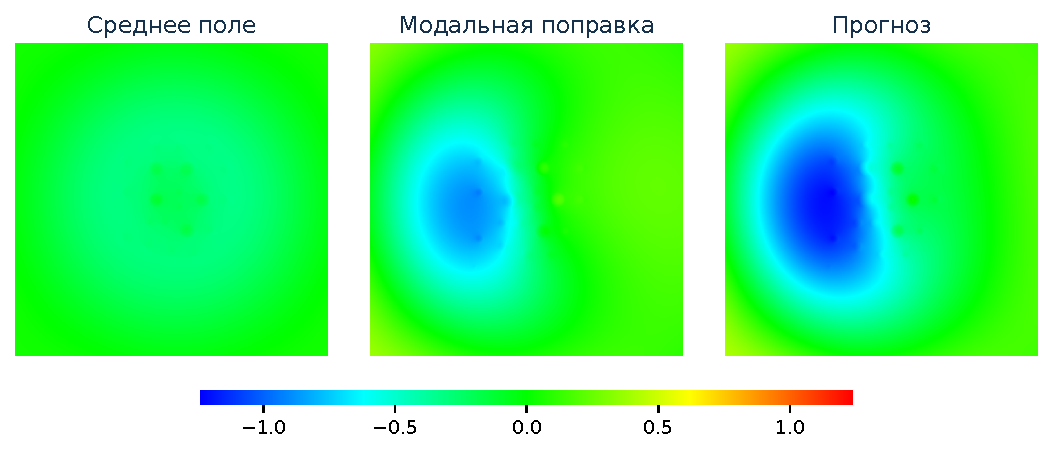
\includegraphics[width=\linewidth]{assets/cover_reconstruction.pdf}
\vspace{1mm}

{\small\sffamily Действительная часть одного прогноза. К среднему полю прибавляется
взвешенная сумма 25 мод на эталонной сетке GMsFEM. Шкала ParaView Blue to Red Rainbow
общая для всех трёх карт. Зелёный цвет соответствует нулю.\par}
\vfill
{\color{teal}\rule{\linewidth}{.8pt}}
{\sffamily\small По материалам проекта \texttt{multiscale-fem-scattering}}\hfill
{\sffamily\small Ноябрь 2026}\par
\end{titlepage}
\color{ink}
\setcounter{page}{2}
\chapter*{Содержание}
\pdfbookmark[0]{Содержание}{contents}
\begingroup
\makeatletter\@starttoc{toc}\makeatother
\endgroup

\vspace{1.1em}
\section*{С чего начать}
\textbf{Для первого чтения} достаточно знать, как умножить матрицу на вектор,
что такое производная и как устроено комплексное число. Найдите на рисунке в главе~\ref{primer:chapter} треугольник
эталонной сетки GMsFEM и восстановите поле в его вершине.
В главе~\ref{walk:chapter} можно повторить этот прогноз в Python.
В разделе~\ref{code:operator} (с.\,\pageref{code:operator}) разберите, как
из матриц слоя получается оператор над коэффициентами поля.

\textbf{Для практикума} пройдите путь от расчётного поля до прогноза
в главах~\ref{math:fem}--\ref{walk:chapter}. Затем попробуйте объяснить
по таблице в главе~\ref{exp:chapter}, сколько точности теряется при сжатии
и сколько добавляет сеть.

\textbf{Для углублённого чтения} обратитесь к главе~\ref{op:chapter}
за условиями устойчивости и оценками ошибки. В главе~\ref{adv:chapter}
показано, что меняется при переходе к комплексному базису и нескольким ветвям сети.

\chapter{Как из поля на сетке получить прогноз}
\label{primer:chapter}

\section{Одна задача и одно поле}
\label{primer:physical}
Представьте, что через неоднородную среду проходит плоская волна.
Мы знаем свойства среды и можем менять направление волны.
Для каждого направления нас интересует одно и то же: каким будет
рассеянное поле в каждой точке области? Один расчёт методом конечных
элементов даёт поле для одного набора условий. Серия таких расчётов
даёт примеры, по которым можно учиться предсказывать следующее поле.

Обозначим набор условий через $p=(A,n,k,\theta)$. Функции $A(x)$ и $n(x)$
задают свойства среды, $k>0$ задаёт волновое число, а $\theta$~--- угол
падения в радианах. Координата $x=(x_1,x_2)$ отвечает на вопрос «где?»,
а набор $p$~--- «при каких условиях?». Если взять две точки при одном $p$,
мы увидим разные значения одного поля. Если изменить $p$ и оставить точку
на месте, получим значение другого поля.

\begin{center}
\begin{tabularx}{\linewidth}{@{}l X@{}}
\toprule
Поле & Как его получить \\ \midrule
Падающее $u_i$ & Вычислить по формуле $u_i(x)=\exp(\ii k\,d\cdot x)$,
где $d=(\cos\theta,\sin\theta)$ и $\ii^2=-1$.\\[2pt]
Рассеянное $u_s$ & Решить краевую задачу или получить приближённый
прогноз обученной модели. Это поле изучается в пособии.\\[2pt]
Полное $u_{\rm tot}$ & Сложить поля как комплексные числа:
$u_{\rm tot}=u_i+u_s$.\\
\bottomrule
\end{tabularx}
\end{center}

Метод конечных элементов (МКЭ, англ.\ FEM) заменяет искомую
функцию набором чисел на сетке. Для линейных треугольных элементов
это значения в узлах $U_i=u_{s,h}(x_i)$, где $h$ характеризует размер
элементов. По ним поле восстанавливается и между узлами:
\[
  u_{s,h}(x)=\sum_{i=1}^{N} U_i\,\varphi_i(x).
\]
Функция $\varphi_i$ равна единице в своём узле и нулю во всех остальных.
Внутри треугольника поле линейно интерполирует значения в трёх вершинах.

\begin{idea}{Какие данные будем разбирать}
В эталонном расчёте GMsFEM область $[-2,2]^2$ содержит 24 включения.
На фоне $A=n=1$, внутри включений $A=0{,}2$ и $n=10$.
В сетке $53\,246$ узлов и $105\,690$ треугольников.
Для этой фиксированной среды сеть по $k$ и $\theta$ предсказывает
50 чисел, по 25 на каждую компоненту комплексного рассеянного поля.
\end{idea}

\clearpage
\section{Как восстановить поле на одном треугольнике}
\label{primer:three-objects}\label{primer:example}
Возьмём тестовый расчёт №\,940 при $k\approx1{,}48616$ и $\theta\approx3{,}30401$.
На рисунке выделен треугольник №\,53227 с вершиной в начале координат.
Номера элементов и узлов соответствуют массивам Python с нумерацией от нуля.

\begin{center}
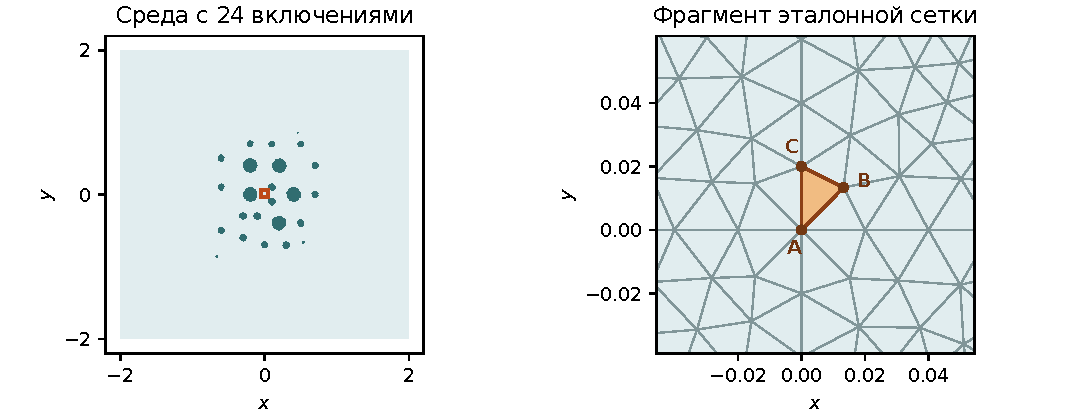
\includegraphics[width=.91\linewidth]{assets/notation_example.pdf}
\captionsetup{hypcap=false}\captionof{figure}{Эталонная геометрия GMsFEM.
Слева тёмным цветом показаны включения, рамкой отмечена область увеличения.
Справа видны рёбра сетки и вершины выбранного элемента.}
\label{primer:figure}
\end{center}

Один \emph{снимок} содержит значения поля сразу во всех узлах.
В каждом узле $i$ усредним действительную часть по 856 обучающим снимкам.
Получим среднее $\mu_i$. Пространственная \emph{мода} $\phi_j$ тоже имеет
значение в каждом узле, но задаёт форму отклонения от среднего.
Для нового запроса сеть выбирает один коэффициент $\widehat c_j$ на всю моду:
\[
 \widehat f_i=\mu_i+\phi_1(x_i)\widehat c_1+
                     \sum_{j=2}^{25}\phi_j(x_i)\widehat c_j .
\]

\begin{center}
\begin{tabular}{@{}lr r r r r r@{}}
\toprule
 & Узел & Среднее & Мода 1$\,\times\widehat c_1$ & Моды 2--25 & Прогноз & МКЭ\\
\midrule
$A$ & 27000 & $-0{,}21008$ & $-0{,}28392$ & $-0{,}04905$ & $-0{,}54305$ & $-0{,}54449$\\
$B$ & 26855 & $-0{,}21080$ & $-0{,}28662$ & $-0{,}03050$ & $-0{,}52792$ & $-0{,}52947$\\
$C$ & 26705 & $-0{,}21035$ & $-0{,}28694$ & $-0{,}04236$ & $-0{,}53966$ & $-0{,}54119$\\
\bottomrule
\end{tabular}
\end{center}

\textbf{Проверка строки $A$.} Сеть дала $\widehat c_1=-0{,}562294$,
а первая мода в этом узле равна $0{,}504940$. Их произведение
равно примерно $-0{,}28392$. Прибавьте среднее и вклад остальных мод:
получится $-0{,}54305$. Последний столбец таблицы получен независимым
способом: для тех же $k,\theta$ решена система МКЭ.

\clearpage
\section{Что известно при новом запросе}
\label{primer:stages}\label{primer:why-svd}
Как сеть получила одно число $\widehat c_1$ для всех трёх вершин?
Рассмотрим, какие величины вычисляют заранее и какие зависят от запроса.

\smallskip\noindent{\sffamily\bfseries\color{navy}1. Решить обучающие задачи}\par\nopagebreak[4]
Для каждого выбранного $p$ метод конечных элементов даёт вектор $U(p)$.
Для проверки качества откладывают отдельные группы данных. Например, при
проверке на новых частотах все направления одной частоты должны попасть
в одну и ту же часть выборки.
\smallskip\noindent{\sffamily\bfseries\color{navy}2. Найти пространственные моды}\par\nopagebreak[4]
По обучающим снимкам вычисляют среднее $\mu$ и матрицу мод
$\Phi=(\phi_1,\ldots,\phi_r)$. Каждая колонка~--- поле на всей сетке.
Такое представление даёт собственное ортогональное разложение
(англ.\ proper orthogonal decomposition, POD). Моды находят с помощью
сингулярного разложения матрицы данных (singular value decomposition, SVD).
При $r$ модах у каждого снимка $r$ коэффициентов.
\smallskip\noindent{\sffamily\bfseries\color{navy}3. Обучить модель коэффициентов}\par\nopagebreak[4]
Модель проекта основана на идее спектрального нейронного оператора
(spectral neural operator, SNO). В выбранном POD-базисе сеть с весами
$\omega$ переводит признаки запроса в коэффициенты
$\widehat c_j$. В ходе обучения $\omega$ меняют так, чтобы восстановленные
поля были близки к расчётным. Среднее поле и моды на этом этапе уже заданы.
\smallskip\noindent{\sffamily\bfseries\color{navy}4. Восстановить новое поле}\par\nopagebreak[4]
По новому набору $p$ сеть выдаёт коэффициенты. После отмены нормировки
выполняют сложение $\widehat f=\mu+\sum_{j=1}^r\phi_j\widehat c_j$.
В базовой модели так восстанавливают отдельно действительную и мнимую части:
$\widehat u_s=\widehat f_R+\ii\widehat f_I$.


\begin{worked}{Проверьте себя}
Изменим только первый коэффициент прогноза на $+0{,}1$. Как изменится
действительная часть поля в вершине $A$? А в других узлах?

\textit{Ответ.} В вершине $A$ добавится $0{,}1\cdot0{,}504940=0{,}050494$.
В каждом другом узле прибавка равна $0{,}1\phi_1(x_i)$. Таким образом,
у коэффициента одно значение на весь снимок, а изменение поля в разных
узлах определяется формой моды.
\end{worked}

В главе~\ref{math:fem} получим уравнение для узлового вектора $U(p)$.
В главе~\ref{math:pod} найдём моды по обучающим снимкам, а в
разделе~\ref{code:operator} разберём, какие матрицы действуют на
коэффициенты внутри нейронного оператора.

\chapter{От плоской волны к конечномерной задаче}
\label{math:fem}
\label{math:chapter}

\section{Падающее, рассеянное и полное поля}
Пусть плоская волна распространяется в однородной среде и встречает
включение с другими свойствами. Мы знаем амплитуду и фазу падающей
волны в каждой точке. Требуется найти, как включение изменяет поле.
Для точки $x=(x_1,x_2)$, волнового числа $k>0$ и угла $\theta$
положим
\begin{align}
 d&=(\cos\theta,\sin\theta),\quad |d|=1,\label{math:direction}\\
 u_i(x)&=\exp(\ii k d\cdot x)
       =\cos(kd\cdot x)+\ii\sin(kd\cdot x).\label{math:incident}
\end{align}
Вектор $d$ задаёт направление распространения. Линии равной фазы
перпендикулярны $d$ и повторяются через длину волны $2\pi/k$ вдоль
этого направления. При принятой временно́й зависимости физическое
колебание имеет вид $\operatorname{Re}(u(x)e^{-\ii\omega t})$.
Модуль комплексного $u$ даёт амплитуду, а аргумент при $u\ne0$ даёт фазу.

Полное поле $u$ складывается из известного падающего поля $u_i$ и
искомого рассеянного поля $u_s$. Именно $u_s$ приближает базовая
нейросетевая модель. Зная приближение $u_{s,h}$, можно вычислить полное
поле в любой точке элемента как $u_i(x)+u_{s,h}(x)$. При интегрировании
этой суммы аналитическую экспоненту вычисляют в точках квадратуры.
Линейная интерполяция суммы узловых значений дала бы другую функцию.

\section{Уравнение для рассеянной волны}
Вычислительная область $\Omega=(-2,2)^2$ окружает неоднородность.
Положительные скалярные коэффициенты $A,n$ ограничены сверху и отделены
от нуля, а в фоновой среде равны единице. Полное поле удовлетворяет
\begin{equation}
 \nabla\cdot(A\nabla u)+k^2nu=0.\label{math:total-pde}
\end{equation}
Для падающего поля $\nabla u_i=\ii k d\,u_i$, откуда
$\Delta u_i+k^2u_i=0$. Подставим $u=u_i+u_s$ в уравнение и воспользуемся
этим тождеством. Тогда
\begin{equation}
 \nabla\cdot(A\nabla u_s)+k^2nu_s
 =\nabla\cdot((1-A)\nabla u_i)+k^2(1-n)u_i.\label{math:scattered-pde}
\end{equation}
Контрасты $1-A$ и $1-n$ задают источник рассеянной волны.
При скачках коэффициентов дивергенцию понимают в смысле распределений.

Чтобы ограничиться квадратом, на его границе $\Gamma=\partial\Omega$
задают приближённое условие выхода волны первого порядка
\begin{equation}
 \partial_\nu u_s=\ii k u_s,\qquad
 \partial_\nu u_s=\nabla u_s\cdot\nu,\label{math:robin}
\end{equation}
где $\nu$ есть внешняя единичная нормаль на стороне квадрата. На данной
стороне это условие точно выполняется для плоской волны, выходящей по её
нормали.
При косом выходе нормальная составляющая волнового вектора меньше $k$,
поэтому искусственная граница может отражать часть волны. Это источник
погрешности ещё до построения сетки.

\section{Слабая форма}
Для вывода обозначим $q=(1-A)\nabla u_i$. Умножим
\eqref{math:scattered-pde} на $\bar v$, где $v\in H^1(\Omega;\C)$,
и проинтегрируем по частям. Черта означает комплексное сопряжение.
Для гладких полей формула Грина даёт
\begin{align}
 -\int_\Omega A\nabla u_s\cdot\nabla\bar v\,dx
 +\int_\Gamma A\partial_\nu u_s\bar v\,ds
 +k^2\int_\Omega nu_s\bar v\,dx
 ={}&-\int_\Omega q\cdot\nabla\bar v\,dx\notag\\
 &+\int_\Gamma(q\cdot\nu)\bar v\,ds
 +k^2\int_\Omega(1-n)u_i\bar v\,dx.\label{math:green}
\end{align}
В окрестности границы $A=1$, поэтому граничный вклад от $q$ исчезает.
Подставив \eqref{math:robin} и умножив обе части на $-1$, получаем
слабую постановку. Найти $u_s\in H^1(\Omega;\C)$, для которого при
каждом $v\in H^1(\Omega;\C)$ выполнено
\begin{align}
 a(u_s,v)&=\ell(v),\label{math:weak}\\
 a(w,v)&=\int_\Omega A\nabla w\cdot\nabla\bar v\,dx
 -k^2\int_\Omega nw\bar v\,dx
 -\ii k\int_\Gamma w\bar v\,ds,\label{math:bilinear}\\
 \ell(v)&=\int_\Omega(1-A)\nabla u_i\cdot\nabla\bar v\,dx
 +k^2\int_\Omega(n-1)u_i\bar v\,dx.\label{math:rhs}
\end{align}
Форма линейна по $w$ и сопряжённо-линейна по $v$. В интегралах
содержатся только первые производные поля и тестовой функции. Такая
запись определена и для кусочно постоянного $A$ со скачками на границах
включений.

\begin{worked}{Проверка правой части}
В однородной среде $A=n=1$, поэтому $\ell(v)=0$ для любого $v$.
При единственности решения имеем $u_s=0$ во всей области, а полное поле
совпадает с падающим. Эта проверка обнаруживает паразитный источник.
Для проверки знака массового вклада возьмём $A=1$ и $n\ge1$, причём
$n>1$ на множестве положительной площади. При $v=u_i$ получаем
$\ell(u_i)=k^2\int_\Omega(n-1)\,dx>0$, поскольку $|u_i|^2=1$.
\end{worked}

\section{Метод конечных элементов на треугольниках}
Разобьём область на треугольники. Узловая базисная функция $\varphi_j$
линейна на каждом элементе, непрерывна и удовлетворяет
$\varphi_j(x_i)=\delta_{ij}$. Пусть $N$ есть число узлов. Ищем приближение
\begin{equation}
 u_{s,h}(x)=\sum_{j=1}^N U_j\varphi_j(x),\qquad
 U=(U_1,\ldots,U_N)^\top\in\C^N.\label{math:fem-expansion}
\end{equation}
Подставим это разложение в \eqref{math:weak} и последовательно возьмём
$v=\varphi_i$, $i=1,\ldots,N$. Получим систему
\begin{align}
 (K-k^2M_n-\ii k B_\Gamma)U&=F,\label{math:fem-system}\\
 K_{ij}&=\int_\Omega A\nabla\varphi_j\cdot\nabla\varphi_i\,dx,
 & (M_n)_{ij}&=\int_\Omega n\varphi_j\varphi_i\,dx,\notag\\
 (B_\Gamma)_{ij}&=\int_\Gamma\varphi_j\varphi_i\,ds,
 & F_i&=\ell(\varphi_i).\notag
\end{align}
Индекс $i$ нумерует уравнения, $j$ нумерует неизвестные.
Матрицы $K,M_n,B_\Gamma$ вещественные и симметричные, каждая имеет
размер $N\times N$. Их комбинация в \eqref{math:fem-system}
комплексно-симметрична и, при ненулевой граничной матрице, неэрмитова.
При неизменных $A,n,k$ и сетке смена направления $d$ меняет только
нагрузку $F\in\C^N$. Для нескольких направлений достаточно одной
факторизации матрицы.

\subsection{Вклад одного элемента}
Пусть на треугольнике $T$ площади $|T|$ коэффициенты равны $A_T,n_T$.
Локальные матрицы жёсткости и массы получают умножением на $A_T$ и $n_T$
соответственно следующих матриц:
\begin{equation}
 (K_T^{(0)})_{ij}=|T|\nabla\varphi_i\cdot\nabla\varphi_j,\qquad
 M_T^{(0)}=\frac{|T|}{12}
 \begin{pmatrix}2&1&1\\1&2&1\\1&1&2\end{pmatrix}.\label{math:local-mass}
\end{equation}
На граничном ребре $e$ длины $L_e$ интегрирование даёт
\begin{equation}
 B_e=\frac{L_e}{6}\begin{pmatrix}2&1\\1&2\end{pmatrix}.\label{math:edge-mass}
\end{equation}
Каждый локальный элемент добавляют к строкам и столбцам общих узлов.
Для правой части из \eqref{math:rhs} аналогично следует
\begin{equation}
 F_{T,j}=(1-A_T)\ii k(d\cdot\nabla\varphi_j)\int_T u_i\,dx
              + k^2(n_T-1)\int_Tu_i\varphi_j\,dx.\label{math:local-rhs}
\end{equation}
В отличие от произведений линейных функций, здесь под знаком интеграла
стоит экспонента. В используемом решателе эти интегралы вычисляются
приближённо, по квадратуре Гаусса с $8\times8$ точками после
преобразования Даффи из квадрата в треугольник.

\begin{worked}{Проверка на единичном прямоугольном треугольнике}
Для вершин $(0,0),(1,0),(0,1)$ базисные функции равны $1-x_1-x_2$, $x_1$,
$x_2$, а площадь равна $1/2$. Их градиенты дают
\[
 K_T^{(0)}=\tfrac12\begin{pmatrix}2&-1&-1\\-1&1&0\\-1&0&1\end{pmatrix}.
\]
Сумма элементов каждой строки равна нулю. Поэтому постоянное поле с
вектором значений $\bm1=(1,1,1)^\top$ имеет нулевую энергию градиента.
Для матрицы массы проверка другая:
$\bm1^\top M_T^{(0)}\bm1=12/24=1/2=\int_T1\,dx$.
\end{worked}

\section{Как измерить ошибку поля}
Пусть $M$ собрана из локальных матриц $M_T^{(0)}$ без коэффициента $n_T$.
Это согласованная матрица массы. Для комплексного вектора $z$ и
соответствующей ему конечно-элементной функции $z_h$ имеем
\begin{equation}
 \|z_h\|_{L^2(\Omega)}^2=z^*Mz,\label{math:consistent-norm}
\end{equation}
где звёздочка обозначает сопряжённое транспонирование. При построении
базиса удобно использовать диагональную матрицу весов $W$, полученную
суммированием строк $M$,
\begin{equation}
 w=M\bm1,\quad W=\diag(w_1,\ldots,w_N),\qquad
 \|z\|_W^2=z^*Wz=\sum_jw_j|z_j|^2.\label{math:lumped-norm}
\end{equation}
Каждый треугольник добавляет $|T|/3$ в вес каждой вершины. Поэтому на
невырожденной сетке $w_j>0$ и $\sum_jw_j=|\Omega|$. Узлы в сгущённой
части сетки получают меньший вес, чем узлы с большой прилегающей площадью.

На предыдущем треугольнике $W_T=I_3/6$. При $z=(1,0,0)^\top$ квадрат
точной нормы равен $1/12$, а квадрат диагональной нормы равен $1/6$.
Обе формы верно интегрируют квадрат константы, однако между узлами
квадрат линейной функции меняется квадратично.

Для $z=a+\ii b$, где $a,b\in\R^N$, симметрия вещественной $M$ даёт
\begin{equation}
 z^*Mz=a^\top Ma+b^\top Mb.\label{math:complex-norm}
\end{equation}
Следовательно, относительная ошибка прогноза $\widehat U$ для
ненулевого эталона $U$ равна
\begin{equation}
 e_M(U,\widehat U)=
 \frac{\|\widehat U-U\|_M}{\|U\|_M}.\label{math:relative-error}
\end{equation}
В этой дроби обе части поля учитываются до извлечения квадратного корня.
При $U=0$ относительная ошибка математически не определена. Для отчётов
принято возвращать ноль при нулевом прогнозе и бесконечность при ненулевом.
Абсолютная ошибка $\|\widehat U-U\|_M$ определена в обоих случаях.

\begin{idea}{Какие данные описывают один расчёт}
Эталон получают, собирая систему по \emph{ячеечным} значениям $A_T,n_T$.
На вход базовой сети поступают \emph{узловые} значения материалов,
полученные арифметическим усреднением по соседним ячейкам. На границе
включения такое усреднение сглаживает скачок. Одно обучающее наблюдение
связывает эти входы и параметры волны с эталонным узловым вектором $U$.
\end{idea}

\chapter{Сжатие поля с помощью POD и SVD}
\label{math:pod}

\section{Среднее поле и пространственные моды}
Пусть $f^{(1)},\ldots,f^{(m)}\in\R^N$ содержат узловые значения
одной вещественной величины на общей сетке. Каждый вектор называют
\emph{снимком}. Например, можно собрать снимки вещественной части
рассеянного поля при разных углах падения. Требуется найти $r$ общих
пространственных функций и представить каждый снимок в виде
\begin{equation}
 f^{(s)}\approx\mu+\Phi c^{(s)},\qquad
 \mu=\frac1m\sum_{s=1}^m f^{(s)},\qquad
 \Phi=(\phi_1,\ldots,\phi_r)\in\R^{N\times r}.\label{math:pod-expansion}
\end{equation}
Здесь $\mu\in\R^N$ хранит среднее по снимкам. Каждый столбец $\phi_j$
задаёт значения одной моды на всей сетке, а $j$-я координата
$c^{(s)}\in\R^r$ задаёт амплитуду этой моды в снимке $s$.
При $r\ll N$ для описания нового поля в том же пространстве достаточно
$r$ чисел. Построение оптимальных по совокупности снимков мод называется
методом главных ортогональных мод (POD, \emph{proper orthogonal
decomposition}). Сингулярное разложение матрицы (SVD, \emph{singular
value decomposition}) даёт способ их вычислить.

\section{От матрицы снимков к базису}
В базовой модели вещественные снимки расположены по строкам матрицы $F$.
Поэтому центрирование и взвешивание имеют вид
\begin{align}
 F&=\begin{pmatrix}(f^{(1)})^\top\\[-2pt]\vdots\\(f^{(m)})^\top\end{pmatrix}
       \in\R^{m\times N},\qquad
 X=F-\bm1_m\mu^\top,\label{math:row-snapshots}\\
 Y&=XW^{1/2},\qquad
 W^{1/2}=\diag(\sqrt{w_1},\ldots,\sqrt{w_N}).\label{math:weighted-snapshots}
\end{align}
В каждом столбце $X$ сумма равна нулю. Поэтому ранг центрированных данных
не превосходит $\min(m-1,N)$. Положительные веса из
\eqref{math:lumped-norm} учитывают площадь, приходящуюся на узел.
Квадратный корень нужен для следующего равенства:
\begin{equation}
 \sum_{s=1}^m\|f^{(s)}-\widehat f^{(s)}\|_W^2
 =\|(F-\widehat F)W^{1/2}\|_F^2.\label{math:weighted-objective}
\end{equation}
Квадрат нормы Фробениуса $\|Y\|_F^2$ есть сумма квадратов модулей всех
элементов матрицы. Взвешивание стоит справа, поскольку номер узла
нумерует столбцы.

Возьмём экономное сингулярное разложение с $q=\min(m,N)$:
\begin{equation}
 Y=U\Sigma V^\top,\qquad
 U\in\R^{m\times q},\quad\Sigma\in\R^{q\times q},\quad
 V\in\R^{N\times q}.\label{math:svd}
\end{equation}
Здесь буква $U$ обозначает матрицу левых сингулярных векторов. Обе
матрицы сингулярных векторов имеют ортонормированные столбцы.
Числа $\sigma_1\ge\ldots\ge\sigma_q\ge0$ на диагонали $\Sigma$
упорядочены по убыванию. Выберем первые $r$ правых сингулярных векторов
$V_r$ и вернёмся к исходным координатам узлов:
\begin{align}
 \Phi&=W^{-1/2}V_r,\label{math:modes}\\
 \Phi^\top W\Phi&=V_r^\top V_r=I_r.\label{math:orthonormal}
\end{align}
Таким образом, столбцы $\Phi$ ортонормированы в метрике $W$.

\subsection{Коэффициенты известного поля}
У известного поля $f$ ищем ближайшее приближение вида $\mu+\Phi c$.
Остаток должен быть $W$-ортогонален каждому столбцу $\Phi$. Из
$\Phi^\top W(f-\mu-\Phi c)=0$ и \eqref{math:orthonormal} следует
\begin{align}
 c_W&=\Phi^\top W(f-\mu),\label{math:encode-column}\\
 P_W f&=\mu+\Phi c_W.\label{math:decode-column}
\end{align}
Вся таблица коэффициентов и восстановленных снимков равна
\begin{align}
 C&=XW\Phi\in\R^{m\times r},\label{math:encode-row}\\
 F_r&=\bm1_m\mu^\top+C\Phi^\top\in\R^{m\times N}.\label{math:decode-row}
\end{align}
На обучающих снимках $C=YV_r=U_r\Sigma_r$. Для нового, ещё неизвестного
рассеянного поля формула \eqref{math:encode-column} недоступна.
Сеть получает параметры задачи и предсказывает коэффициенты, после чего
восстанавливается узловой вектор.

\section{Пример с двумя узлами}
Возьмём три снимка с двумя координатами и назначим второму узлу
вчетверо больший вес:
\begin{equation}
 F=\begin{pmatrix}0&0\\1&1\\2&2\end{pmatrix},\qquad W=\diag(1,4).
 \label{math:example-data}
\end{equation}
Вычитая среднее $\mu=(1,1)^\top$ и умножая вторую координату на $2$,
получаем
\[
 Y=\begin{pmatrix}-1&-2\\0&0\\1&2\end{pmatrix}
 =\begin{pmatrix}-1\\0\\1\end{pmatrix}\begin{pmatrix}1&2\end{pmatrix}.
\]
Матрица имеет ранг один. Единственное положительное сингулярное число
равно произведению длин этих двух векторов, $\sigma_1=\sqrt{10}$.
Правый сингулярный вектор равен $(1,2)^\top/\sqrt5$. Поэтому мода
$\phi=W^{-1/2}V_1=(1,1)^\top/\sqrt5$ и
$\phi^\top W\phi=(1+4)/5=1$. Три коэффициента равны $-\sqrt5$, $0$ и
$\sqrt5$. Например, из последнего получаем
$\mu+\sqrt5\,\phi=(2,2)^\top$, как в последней строке $F$.

\begin{worked}{Задача. Спроецируйте новое поле}
Для $f=(2,0)^\top$ найдите ближайшее поле $P_W f$ на той же прямой.
Проверьте ортогональность остатка.

\textbf{Решение.} Отклонение от среднего равно $(1,-1)^\top$, поэтому
$c_W=(1-4)/\sqrt5=-3/\sqrt5$. Реконструкция имеет равные координаты
$P_W f=(2/5,2/5)^\top$. Остаток $e=(8/5,-2/5)^\top$ удовлетворяет
$\phi^\top We=(8/5-8/5)/\sqrt5=0$. Квадрат его нормы равен $16/5$.
Второй узел получил больший вес, и общее значение $2/5$ оказалось
ближе к нулю во втором узле, чем к двум в первом.
\end{worked}

\section{Что оптимизирует усечение SVD}
Для точного SVD теорема Эккарта--Янга даёт
\begin{equation}
 \min_{\operatorname{rank}(Z)\le r}\|Y-Z\|_F^2
 =\sum_{j>r}\sigma_j^2.\label{math:eckart-young}
\end{equation}
В силу \eqref{math:weighted-objective} это минимальная сумма квадратов
\emph{абсолютных} ошибок на обучающих снимках в метрике $W$ при фиксированном
среднем. Для $E=\|Y\|_F^2>0$ доля сохранённой энергии отклонений равна
\begin{equation}
 \eta_r=\frac{\sum_{j\le r}\sigma_j^2}{E},\qquad
 \frac{\|(F-F_r)W^{1/2}\|_F}{\|XW^{1/2}\|_F}
 =\sqrt{1-\eta_r}.\label{math:energy}
\end{equation}
Например, $99\,\%$ энергии дают $10\,\%$ относительной ошибки для всей
матрицы \emph{центрированных} снимков в этой норме. У отдельного поля
со своим знаменателем ошибка может оказаться больше или меньше.
При $E=0$ все снимки совпадают со средним и достаточно ранга ноль.

Для произвольных предсказанных коэффициентов $\widehat c$ ортогональность
остатка даёт точное разложение
\begin{equation}
 \|f-\mu-\Phi\widehat c\|_W^2
 =\|f-P_W f\|_W^2+\|c_W-\widehat c\|_2^2.\label{math:pythagoras}
\end{equation}
Первый член уже фиксирован выбранным пространством. Обучение сети может
изменить второй. Если качество поля оценивают в точной конечно-элементной
норме $M$, ближайшие коэффициенты определяют заново:
\begin{equation}
 Gc_M=\Phi^*M(f-\mu),\qquad G=\Phi^*M\Phi.\label{math:consistent-projection}
\end{equation}
При независимых столбцах $\Phi$ и положительно определённой $M$ матрица
Грама $G$ положительно определена. Для $P_M f=\mu+\Phi c_M$ из той же
ортогональности следует разложение с $\|c_M-\widehat c\|_G^2$ вместо
евклидовой нормы коэффициентов. Именно $\|f-P_M f\|_M$ даёт наименьшую
достижимую ошибку поля в выбранном пространстве. Сравнение обеих
проекций доказано в разделе~\ref{rig:projection}.

\section{Два способа представить комплексное поле}
В базовой модели четыре вещественных базиса строятся отдельно для входных
материалов $A,n$ и для выходных полей $\operatorname{Re}u_s$,
$\operatorname{Im}u_s$. У каждого свое среднее, свой ранг и своя таблица
мод. Совпадение номера столбца между двумя таблицами само по себе
не связывает пространственные функции. При прогнозе поле собирается как
\begin{equation}
 \widehat u_s=\mu_R+\Phi_R\widehat c_R+
             \ii(\mu_I+\Phi_I\widehat c_I).\label{math:complex-decode}
\end{equation}
При этом $\widehat c_R\in\R^{r_R}$, $\widehat c_I\in\R^{r_I}$,
а ошибка поля учитывает обе компоненты по \eqref{math:complex-norm}.

Для комплексного POD удобно расположить \emph{центрированные снимки по
столбцам} матрицы $S\in\C^{N\times m}$. Пусть $M=R^*R$ положительно
определена, например $R$ есть верхний треугольный множитель Холецкого.
Если $RS=Q\Sigma V^*$, то
\[
 \Phi=R^{-1}Q_r,\qquad \Phi^*M\Phi=I_r,\qquad
 c=\Phi^*M(f-\mu)\in\C^r.
\]
Теперь одна мода может одновременно описывать изменения амплитуды и фазы.
Знак вещественной моды произволен. Для комплексной моды можно изменить
фазу $\phi_j\mapsto e^{\ii\alpha}\phi_j$ и компенсировать её заменой
$c_j\mapsto e^{-\ii\alpha}c_j$. При кратном сингулярном числе допустим
унитарный поворот внутри соответствующего подпространства. Поэтому при
сравнении вычислений проверяют поля или проекторы.

\section{Как выбрать ранг по данным}
Материалы одной среды могут повторяться при разных углах и частотах. В
обучающую матрицу материалов берут по одному снимку от каждой среды,
а для выходных полей используют все обучающие решения. При фиксированном
материале его центрированные снимки нулевые, и входной ранг равен нулю.
Тогда известную среду представляет одно среднее. Информацию о меняющихся
частоте и направлении передают оставшиеся входные координаты.

Для выходных полей базовая модель перебирает ранги от единицы до заданного
предела. Для обучения нужна хотя бы одна выходная мода. Если обе
компоненты постоянны по снимкам, каждую из них уже описывает её среднее.
При каждом ранге известные поля проверочной выборки проецируют в метрике
$W$, восстанавливают обе компоненты и усредняют относительную ошибку
\eqref{math:relative-error} в метрике $M$. Берут первый ранг, при котором
средняя ошибка не превышает заданного порога. Если такого ранга нет,
оставляют наибольший доступный и отмечают, что порог не достигнут.
У компоненты с меньшим численным рангом сохраняют только имеющиеся моды.
Нулевые столбцы, которые могут добавлять при хранении, в матрицу Грама
\eqref{math:consistent-projection} не включают.

\begin{idea}{Три числа для трёх вопросов}
Остаток по спектру \eqref{math:energy} показывает, сколько вариации потеряно
при сжатии обучающих данных. Ошибка проекции проверочного поля показывает,
насколько подходит пространство для новых условий. Ошибка прогноза на
независимом тесте дополнительно учитывает выбор коэффициентов нейросетью.
Среднее и моды следует вычислять только по обучающим данным. Включение
тестового поля в SVD заранее сообщает методу о пространственных
особенностях этого поля.
\end{idea}

\subsection{Численный ранг и приближённое разложение}
Полное экономное SVD вычисляет все $q$ сингулярных чисел. Для большого
числа снимков можно приближённо найти ведущие направления. Пусть $t$
есть запрошенный ранг, ограниченный сверху числом $q$. При $t=0$ или
нулевой энергии центрированных снимков базис сразу оставляют пустым.
В остальных случаях при $t+10<q$
используемый случайный алгоритм берёт гауссову матрицу
$\Omega_g\in\R^{N\times(t+10)}$ и строит ортонормированный базис $Q$
по столбцам $Y\Omega_g$. Чтобы лучше выделить ведущие направления,
дважды выполняются шаги
\begin{equation}
 Z=\operatorname{orth}(Y^\top Q),\qquad
 Q=\operatorname{orth}(YZ),\label{math:power}
\end{equation}
где $\operatorname{orth}$ оставляет ортонормированные столбцы из
экономного QR-разложения. Затем находят SVD меньшей матрицы $Q^\top Y$.
При $t+10\ge q$ применяется полное экономное разложение.
У приближённых мод измеряют фактическую ошибку восстановления:
равенство с оптимальным хвостом спектра доказано для точного SVD.

Для обоих алгоритмов отсеивают сингулярные числа ниже численного
разрешения. В данной реализации сохраняют числа, которые строго
превышают
\begin{equation}
 \tau=\epsilon_{64}\max(m,N)\max\bigl(\sigma_1,\|FW^{1/2}\|_F\bigr).
 \label{math:numeric-threshold}
\end{equation}
Здесь $\epsilon_{64}$ есть машинная точность, а $\sigma_1$ берётся из
вычисленного разложения. Масштаб до вычитания среднего важен для почти
постоянных полей: малое отклонение от большого фона может быть целиком
обусловлено округлением.

\chapter{Спектральный нейронный оператор Фанаскова и Оселедца}
\label{sno:chapter}

Пусть оператор $\mathcal G$ каждой входной функции $f$ сопоставляет
выходную функцию $g$. В спектральном нейронном операторе
(\emph{Spectral Neural Operator}, SNO) Фанаскова и Оселедца обе функции
представлены конечными рядами. Чтобы приближать $\mathcal G$,
достаточно научиться по коэффициентам первого ряда определять
коэффициенты второго. Авторы рассматривают полиномы Чебышёва и ряды
Фурье. Разберём сначала полиномиальный случай.
Общее определение дано в
\href{https://arxiv.org/html/2205.10573v2\#S4}{разделе~4 статьи, формула (3)},
а устройство сети --- в приложении~C.1.3, формулы (19)--(22).

\section{Коэффициенты входной и выходной функций}
\label{sno:bases}

На отрезке $[-1,1]$ положим $T_j(\cos t)=\cos(jt)$.
Первые три полинома Чебышёва равны $T_0=1$, $T_1=x$ и $T_2=2x^2-1$.
Условимся записывать ряд в виде $f_p=\sum_{j=0}^p d_j T_j$.
Тогда, например,
\[
 f(x)=1+x+x^2=\tfrac32T_0(x)+T_1(x)+\tfrac12T_2(x),
 \qquad d=(3/2,1,1/2)^\top .
\]
При $x=0$ имеем $T_2(0)=-1$, и ряд даёт исходное значение $f(0)=1$.

Ортогональность полиномов с весом $\rho(x)=(1-x^2)^{-1/2}$
определяет способ вычисления $d$. Если
$h_j=\int_{-1}^1 T_j(x)^2\rho(x)\,dx$, то
\begin{equation}
 d_j=\frac{1}{h_j}\int_{-1}^1 f(x)T_j(x)\rho(x)\,dx,
 \qquad h_0=\pi,\quad h_j=\pi/2\ (j\ge1).
 \label{sno:cheb-coefficients}
\end{equation}
Для полинома степени не выше $p\ge1$ те же числа восстанавливаются
по значениям в $p+1$ узлах $x_m=\cos(\pi m/p)$.
Например, при $p=2$ значения $f(1)=3$, $f(0)=1$, $f(-1)=1$ дают
$d_0+d_1+d_2=3$, $d_0-d_2=1$ и $d_0-d_1+d_2=1$.
Из первой и третьей строк получаем $d_1=1$, а из двух оставшихся
условий $d_0+d_2=2$ и $d_0-d_2=1$ находим $d_0=3/2$ и $d_2=1/2$.
Для произвольной непрерывной функции значения в этих узлах определяют
интерполирующий полином. Его коэффициенты могут отличаться от интегралов
\eqref{sno:cheb-coefficients}.

Обозначим извлечение $p+1$ входных коэффициентов через $E_p$, а
вычисление выходного ряда через $D_r$. Сеть $N_\vartheta$
определяет приближённый оператор
\begin{equation}
 f\ \xrightarrow{E_p}\ d\in\R^{p+1} \xrightarrow{N_\vartheta}\ \widehat b\in\R^{r+1} \xrightarrow{D_r}\ \widehat g(x)=\sum_{i=0}^{r}\widehat b_i T_i(x).
 \label{sno:operator-factorization}
\end{equation}
Степени $p$ и $r$ выбираются отдельно. При обучении известны пары
$(f,g)$, следовательно, доступны входные и эталонные выходные
коэффициенты. По этим парам подбирают общие веса $\vartheta$.
Для новой функции $f$ веса уже зафиксированы, а $\widehat b$
вычисляется заново. После этого $\widehat g$ можно вычислить в любой
точке отрезка. Число степеней свободы ряда при сгущении сетки остаётся
равным $r+1$.

Пусть, например, требуется учиться дифференцированию полиномов степени
не выше двух. Производные первых трёх мод равны $0$, $T_0$ и $4T_1$,
поэтому эталонное отображение коэффициентов в этой задаче известно:
\[
 b=\begin{pmatrix}0&1&0\\0&0&4\end{pmatrix}d .
\]
Входу $(3/2,1,1/2)^\top$ соответствует метка $(1,2)^\top$.
Её декодирование даёт $g(x)=1+2x$, то есть производную исходного
полинома. На такой паре можно проверить сразу оба преобразования
и смысл регрессии: для этого входа сеть должна приблизить числа 1 и 2.

Для периодической функции периода~2 ту же схему задают
$g_\nu(x)=e^{\ii\pi\nu x}$, $|\nu|\le K$. В этой нормировке
$d_\nu=\tfrac12\int_{-1}^1f(x)e^{-\ii\pi\nu x}\,dx$.
Для тригонометрического полинома с указанной полосой интеграл можно
заменить дискретным средним. Если $J=2K+1$ и $x_m=-1+2m/J$, то
\[
 d_\nu=\frac1J\sum_{m=0}^{J-1}f(x_m)e^{-\ii\pi\nu x_m}.
\]
Например, у $f(x)=\cos(\pi x)$ коэффициенты $d_{-1}=d_1=1/2$,
а остальные равны нулю. Это частный случай симметрии
$d_{-\nu}=\overline{d_\nu}$ для вещественных функций. Авторский код
пользуется этой симметрией и хранит неотрицательные частоты
\href{https://github.com/VLSF/SNO/blob/4362226284f22f6f456d429ec4ddec5b8596e894/functions/Fourier.py\#L43-L56}{(прямое и обратное преобразования)}.

\section{Как один слой действует на функции}
\label{sno:mixed-layer}

Пусть на входе слоя $\ell$ функций, каждая представлена $k$ модами.
Запишем их коэффициенты в матрицу $U\in\R^{k\times\ell}$.
Столбец задаёт одну функцию, а строка собирает вклад одной моды во
всех функциях. Внутри сети такие функции называют скрытыми каналами.
Разные примеры обучающей выборки имеют отдельные матрицы $U$.

Исходная сеть состоит из трёх подсетей $N_3\circ N_2\circ N_1$.
\[
 \underbrace{U}_{\text{входные каналы}}
 \xrightarrow{N_1}
 \underbrace{V}_{\text{скрытые каналы}}
 \xrightarrow{N_2}
 \underbrace{Y}_{\text{новые моды и каналы}}
 \xrightarrow{N_3}
 \underbrace{\widehat U}_{\text{выходные каналы}} .
\]
В $N_1$ и $N_3$ каналы смешиваются одинаково для каждой строки:
$U^+=\sigma(UC+\bm 1 a^\top)$, где
$C\in\R^{\ell\times m}$, $a\in\R^m$, $\bm 1\in\R^k$.
Такое смещение сдвигает каждый коэффициент данного канала на одно и то же число.
Например, прибавление $a$ к обеим модам $T_0,T_1$ добавляет к
восстановленной функции $a+ax$. В $N_2$ добавляется матрица $B$,
связывающая разные моды. Типовой
внутренний слой статьи имеет вид
\begin{equation}
 U^+=\sigma(BUC+\beta),\qquad
 B\in\R^{s\times k},\quad
 C\in\R^{\ell\times m},\quad
 \beta\in\R^{s\times m}.
 \label{sno:paper22}
\end{equation}
Здесь $C$ обозначает матрицу $A$ из формулы (22) статьи.
Умножение справа меняет число каналов с $\ell$ на $m$,
умножение слева --- число мод с $k$ на $s$.
Каждое выходное число до активации равно
\[
 z_{i\gamma}=\sum_{j=1}^k\sum_{\alpha=1}^{\ell}
         B_{ij}U_{j\alpha}C_{\alpha\gamma}+\beta_{i\gamma}.
\]
Тем самым один слой задаёт веса вида $B_{ij}C_{\alpha\gamma}$.
При записи $U$ столбец за столбцом его линейная часть имеет матрицу
$C^\top\otimes B$, составленную из блоков $C_{\alpha\gamma}B$.
Слой содержит $sk+\ell m+sm$ обучаемых вещественных чисел, включая
смещение. Аффинное отображение с отдельным весом для каждой пары
входной и выходной координат потребовало бы $(k\ell)(sm)+sm$ чисел.

\clearpage
\textbf{Пример.}
Пусть базис состоит из $T_0,T_1$, а два входных канала представляют
функции $1$ и $2x$. Выберем для учебного расчёта
\[
 U=\begin{pmatrix}1&0\\0&2\end{pmatrix},\quad
 C=\begin{pmatrix}1&-1\\1&1\end{pmatrix},\quad
 B=\begin{pmatrix}1&1\\1&-1\end{pmatrix},\quad
 \beta=\begin{pmatrix}0&0\\1&0\end{pmatrix}.
\]
После умножения справа и смешивания мод получаем
\[
 UC=\begin{pmatrix}1&-1\\2&2\end{pmatrix},
 \qquad BUC=\begin{pmatrix}3&1\\-1&-3\end{pmatrix},
 \qquad Z=BUC+\beta=\begin{pmatrix}3&1\\0&-3\end{pmatrix}.
\]
Применим поэлементно $s(t)=\log(1+e^t)$ (softplus). Тогда
\[
 U^+=s(Z)\approx\begin{pmatrix}3{,}04859&1{,}31326\\0{,}69315&0{,}04859\end{pmatrix}.
\]
Первый выходной канал есть $3{,}04859+0{,}69315x$. В точке $x=1$
он принимает значение $3{,}74174$. Число $0{,}69315$ в нижней строке
определяет наклон этой функции. Так по одной записи $U^+$
можно отдельно проверить вычисление слоя и восстановление функции.

В авторской программе последний слой \emph{каждой} подсети возвращает
аффинный результат $Z$ без активации. Для комплексных каналов внутри подсети
используется $s(\operatorname{Re}z)+\ii s(\operatorname{Im}z)$.
При обучении усредняют нормы Фробениуса ошибок таблиц по примерам.
Вычисление нормы состоит из суммирования квадратов модулей ошибок
коэффициентов и извлечения квадратного корня. Для отчётных метрик
статьи функции восстанавливают на общей равномерной сетке
(приложение~C.3).
\href{https://github.com/VLSF/SNO/blob/4362226284f22f6f456d429ec4ddec5b8596e894/architectures/SNO_1D.py}{Вещественный}
и
\href{https://github.com/VLSF/SNO/blob/4362226284f22f6f456d429ec4ddec5b8596e894/architectures/fSNO_1D.py}{комплексный код для случая 1D}.

\section{Связь матрицы мод с интегральным оператором}

Почему обычная матрица $B$ описывает оператор, действующий на функции?
Рассмотрим один канал в базисе Чебышёва, с нумерацией мод от нуля.
Линейное преобразование $d\mapsto Bd$ определяет функцию
$(\mathcal B f)(x)=\sum_{i,j} T_i(x)B_{ij}d_j$.
Подставив интеграл \eqref{sno:cheb-coefficients} и вынеся конечную
сумму под знак интеграла, получим
\begin{equation}
 (\mathcal B f)(x)=\int_{-1}^1 K_B(x,y)f(y)\rho(y)\,dy,
 \qquad
 K_B(x,y)=\sum_{i,j} T_i(x)B_{ij}\frac{T_j(y)}{h_j}.
 \label{sno:kernel}
\end{equation}
Таким образом, элементы матрицы задают коэффициенты ядра в двух
пространственных переменных. Образ $\mathcal B$ лежит в линейной
оболочке выходных полиномов. Ограничение числа мод одновременно
ограничивает ранг оператора.

Положение нелинейности тоже имеет значение. Возведение функции
$f(x)=\cos(\pi Kx)$ в квадрат порождает гармонику $2K$, поскольку
$f^2=(1+\cos(2\pi Kx))/2$. Возьмём $J=2K+1$ и узлы $x_m=2m/J$,
$m=0,\ldots,J-1$, на одном периоде. В этих узлах
$e^{\ii\pi(2K)x_m}=e^{-\ii\pi x_m}$, поскольку множитель
$e^{\ii \pi J x_m}$ равен 1. Поэтому высокую гармонику невозможно
отличить по отсчётам от гармоники с номером $-1$. Это наложение
частот (\emph{aliasing}) при дискретизации. В слое~\eqref{sno:paper22}
нелинейность применяется непосредственно к числам таблицы. После
неё ряд имеет ровно столько позиций, сколько строк в $U^+$.
Если истинный ответ содержит отброшенные моды, ошибка усечения
сохраняется даже при точном прогнозе всех оставленных коэффициентов.

В SVD-SNO v2 моды строятся по обучающим полям методом POD.
В блоке появляются локальное преобразование каналов и остаточная
связь (глава~\ref{code:implementation}).

\chapter{Как устроена модель SVD-SNO v2}
\label{code:implementation}

Для одного примера известны два узловых поля материала $A,n\in\R^N$,
угол $\theta$ и волновое число $k$. Требуется восстановить комплексное
поле $u_s\in\C^N$ в тех же узлах. Эталонные поля даёт расчёт методом
конечных элементов. В репозитории объект \texttt{Predictor} сначала
кодирует входные данные, вызывает коэффициентную сеть \texttt{SVDSNO},
затем восстанавливает поле. Рассмотрим версию архитектуры~2.

\section{Представление данных и выбор ранга}
\label{code:preprocessing}

По обучающей выборке строят четыре вещественных базиса для $A$, $n$,
$u_R=\operatorname{Re}u_s$ и $u_I=\operatorname{Im}u_s$.
Для каждого поля $v$ сохраняют его среднее $\mu_v\in\R^N$ и матрицу
мод $\Phi_v\in\R^{N\times r_v}$, где $r_v$ --- число оставленных мод.
Для входных базисов берут по одному снимку каждой обучающей среды,
чтобы число запросов к среде не определяло её вес в POD. Для выходных
базисов берут все обучающие поля рассеяния. Диагональную матрицу узловых
весов $W=\diag(M\bm 1)$ получают из сумм строк согласованной матрицы
масс $M$. В этой метрике имеем
\begin{equation}
 \Phi_v^\top W\Phi_v=I,\qquad
 c_v=\Phi_v^\top W(v-\mu_v),\qquad
 v_r=\mu_v+\Phi_v c_v .
 \label{code:pod-encoding}
\end{equation}
Если все обучающие среды одинаковы, центрированные входные снимки
нулевые и оба входных ранга равны нулю. Сами $A,n$ при этом могут
существенно меняться от узла к узлу.

Длину выходной таблицы $r_{\rm out}$ выбирают по валидационной выборке
$V$. Кандидаты $r$ идут от 1 до максимального доступного ранга двух
выходных базисов. В каждой компоненте используют первые $r$ мод или
весь базис, если его ранг меньше. Коэффициенты находят по формуле
\eqref{code:pod-encoding} с весами $W$, а комплексную реконструкцию
$u^{(t)}_{s,r}$ оценивают в норме $M$:
\begin{equation}
 E_V(r)=\frac{1}{|V|}\sum_{t\in V}
 \frac{\norm{u_s^{(t)}-u^{(t)}_{s,r}}_M}{\norm{u_s^{(t)}}_M},
 \qquad \norm{v}_M^2=v^*Mv .
 \label{code:rank-criterion}
\end{equation}
Выбирают первый ранг, при котором средняя ошибка не превышает
заданного порога. Если порог недостижим, оставляют наибольший доступный
ранг и сохраняют признак этого случая. У вещественного и мнимого
базисов итоговые ранги $r_R,r_I$ могут различаться. Для более короткого
базиса недостающие столбцы при восстановлении поля считаются нулевыми.
Критерий~\eqref{code:rank-criterion} характеризует точность представления
на валидации, до обучения коэффициентной сети.

\section{Из входных признаков в коэффициенты поля}
\label{code:network}

Входные POD-коэффициенты и волновое число нормируют с помощью средних
и стандартных отклонений обучающей выборки. Каждый признак $x$
преобразуют по правилу $\widetilde x=(x-m)/s$, где $m$ и $s$ ---
среднее и стандартное отклонение значений этого признака по обучающим
примерам. Для почти постоянного признака код принимает $s=1$.
Вектор признаков одной задачи равен
\begin{equation}
 f=(\widetilde c_A,\widetilde c_n,\cos\theta,\sin\theta,\widetilde k)
       \in\R^{r_A+r_n+3}.
 \label{code:feature-vector}
\end{equation}
Функция \path{coefficient_tokens} превращает его в таблицу из
$R=\max(r_A,r_n,r_{\rm out})$ строк и пяти столбцов:
\begin{equation}
 T_{j,:}=(a_j,\eta_j,\cos\theta,\sin\theta,\widetilde k),\qquad
 1\le j\le R .
 \label{code:tokens}
\end{equation}
Последовательность $a$ содержит $\widetilde c_A$ и затем нули до
длины~$R$. Так же, независимо, дополняют $\widetilde c_n$, получая $\eta_j$.
Индекс строки $j$ указывает позицию в каждой последовательности.
Базисные функции, стоящие на этой позиции у $A$ и $n$, могут различаться.
Угловые признаки сохраняют периодичность $\theta$ и доступны каждой строке.
Например, при $r_A=3$, $r_n=1$ и $r_{\rm out}=2$ получаем $R=3$.
В первые два столбца записывают
$a=(\widetilde c_{A,1},\widetilde c_{A,2},\widetilde c_{A,3})^\top$
и $\eta=(\widetilde c_{n,1},0,0)^\top$. Третий коэффициент $A$
может влиять на первые две строки через смешивание модальных позиций.

Каждую строку переводят из пяти чисел в $H$ скрытых признаков:
$Z_0=\GELU(TW_0+\bm 1 b_0^\top)$, где $W_0\in\R^{5\times H}$,
$b_0\in\R^H$, а $\bm 1$ --- столбец из $R$ единиц.
Здесь и далее $\GELU(t)=t\,\mathbb P(\xi\le t)$ для
$\xi\sim\mathcal N(0,1)$ действует поэлементно. Далее сеть применяет
$L$ блоков с разными наборами весов. Для одного блока имеем
\begin{equation}
 Z^+=Z+\GELU\bigl(ZW_{\rm loc}+\bm 1 b^\top+BZ W_{\rm ch}\bigr),
 \qquad Z,Z^+\in\R^{R\times H}.
 \label{code:block}
\end{equation}
Матрицы $W_{\rm loc},W_{\rm ch}\in\R^{H\times H}$ действуют справа на
каналы. Матрица $B\in\R^{R\times R}$ действует слева на модальные
позиции. Первая ветвь преобразует каждую строку отдельно. Во второй
ветви результат для позиции $j$ зависит от других строк через $B_{ji}$.
Слагаемое $Z$ переносит исходную таблицу в следующий слой
(рис.~\ref{code:block-diagram}).
В PyTorch матрица слоя \texttt{Linear} действует по последней оси,
поэтому для применения $B$ код временно меняет местами оси строк и каналов.

\begin{figure}[htbp]
\centering
\begin{tikzpicture}[
  stage/.style={draw=teal,fill=soft,rounded corners=2pt,align=center,
                minimum height=7mm,inner xsep=2.5mm,font=\small},
  sum/.style={circle,draw=teal,fill=soft,inner sep=1pt,minimum size=5mm},
  wire/.style={-{Stealth[length=2mm]},semithick,draw=navy},
  route/.style={semithick,draw=navy}]
  \node (z) at (0,0) {$Z$};
  \node[stage] (local) at (3,0.66) {$ZW_{\rm loc}+\bm 1b^\top$};
  \node[stage] (mixed) at (3,-0.66) {$B(ZW_{\rm ch})$};
  \node[sum] (sum) at (5.25,0) {$+$};
  \node[stage] (gelu) at (6.7,0) {$\GELU$};
  \node[sum] (add) at (8.25,0) {$+$};
  \node (out) at (9.5,0) {$Z^+$};
  \coordinate (skip) at (0.75,0);
  \coordinate (split) at (1.40,0);
  \coordinate (merge) at (4.65,0);
  \draw[route] (z) -- (split);
  \fill[navy] (skip) circle (1.4pt);
  \fill[navy] (split) circle (1.4pt);
  \draw[wire] (split) |- (local.west);
  \draw[wire] (split) |- (mixed.west);
  \draw[wire] (local.east) -| (merge) -- (sum.west);
  \draw[route] (mixed.east) -| (merge);
  \draw[wire] (sum) -- (gelu);
  \draw[wire] (gelu) -- (add);
  \draw[wire] (skip) -- (0.75,-1.35) -- (8.25,-1.35) -- (add.south);
  \draw[wire] (add) -- (out);
  \node[font=\small\sffamily,text=navy,below] at (4.5,-1.35) {Остаточная связь};
\end{tikzpicture}
\caption{Две ветви блока сначала суммируются. После GELU к результату
прибавляется входная таблица. Размер каждой таблицы равен $R\times H$.}
\label{code:block-diagram}
\end{figure}

Общее для строк аффинное отображение $H\to 2$ применяется к первым
$r_{\rm out}$ строкам $Z_L$. В строке $j$ оно вычисляет
$\widehat q_{j,:}=(Z_L)_{j,:}W_{\rm out}+b_{\rm out}^\top$, где
$W_{\rm out}\in\R^{H\times 2}$ и $b_{\rm out}\in\R^2$.
Два столбца $\widehat q_{j,\alpha}$, $\alpha\in\{R,I\}$, задают
коэффициенты в нормированных единицах.
Для каждой моды и компоненты хранятся отдельные среднее $m_{j,\alpha}$
и масштаб $s_{j,\alpha}$. Декодер вычисляет
\begin{align}
 \widehat c_{j,\alpha}&=m_{j,\alpha}+s_{j,\alpha}\widehat q_{j,\alpha},
                         \label{code:denormalize}\\
 \widehat u_\alpha&=\mu_\alpha+\Phi_\alpha\widehat c_\alpha,
 \qquad \widehat u_s=\widehat u_R+\ii\widehat u_I .
                         \label{code:decode-physical}
\end{align}
В произведении на $\Phi_\alpha$ участвуют только $r_\alpha$ активных
коэффициентов. Каждая из двух сумм использует собственные моды и среднее.

\section{Как считать ошибку поля по коэффициентам}
\label{code:fem-loss}

При обучении важна величина $\norm{\widehat u_s-u_s}_M$. Прямой расчёт
требовал бы восстанавливать $N$ узловых значений для каждого примера
на каждом шаге. Ту же величину можно получить из квадратичных форм
порядка $r_R$ и $r_I$ и заранее вычисленных остатков двух компонент.

Для одной вещественной компоненты положим $y=u-\mu$,
$G=\Phi^\top M\Phi$. При линейно независимых активных столбцах
$\Phi$ матрица $G$ положительно определена, поскольку
$v^\top Gv=\norm{\Phi v}_M^2>0$ при $v\ne0$. Для наилучшей проекции
минимизируем $\norm{y-\Phi c}_M^2$ по $c$. Приравнивая производную
к нулю, получаем уравнение для $c_*$ и определяем остаток $\rho$:
\begin{equation}
 G c_* =\Phi^\top M y,\qquad \rho=y-\Phi c_* .
 \label{code:consistent-projection}
\end{equation}
Из нормальных уравнений следует $\Phi^\top M\rho=0$. Запишем ошибку
в виде $\widehat u-u=\Phi(\widehat c-c_*)-\rho$ и раскроем квадрат.
Смешанное слагаемое исчезает в силу ортогональности. Получается
\begin{equation}
 \norm{\widehat u-u}_M^2
   =(\widehat c-c_*)^\top G(\widehat c-c_*)+\norm{\rho}_M^2 .
 \label{code:quadratic-identity}
\end{equation}
Первое слагаемое обращается в нуль при точном прогнозе оптимальных
коэффициентов. Второе даёт наименьший достижимый квадрат нормы ошибки
для данного примера и базиса. При нулевом ранге остаётся только ошибка
относительно среднего поля. Формула~\eqref{code:pod-encoding} даёт
коэффициенты проекции с диагональным весом $W$, тогда как $c_*$ и $G$
определяются скалярными произведениями в метрике $M$.

Матрица $M$ вещественна и симметрична, поэтому квадрат комплексной
нормы равен сумме квадратов норм двух компонент. Для примера $t$
обозначим через $e_t$ сумму правых частей~\eqref{code:quadratic-identity}
по $R,I$, а через $d_t=\norm{u_s^{(t)}}_M^2$ --- энергию эталона.
При положительных энергиях обычного масштаба функция потерь в группе
$J$ примеров равна $|J|^{-1}\sum_{t\in J}\sqrt{e_t/d_t}$.
Вблизи нуля реализация использует
\begin{equation}
 \mathcal L_J=\frac1{|J|}\sum_{t\in J}
 \frac{e_t}{\sqrt{\max(e_t,\varepsilon)}\sqrt{\max(d_t,\varepsilon)}},
 \qquad \varepsilon=10^{-24},\quad e_t\ge0 .
 \label{code:stable-loss}
\end{equation}
Энергии остатка вычисляют непосредственно по $\rho$, чтобы избежать
потери точности при вычитании близких энергий. Величины $c_*$,
$\norm{\rho}_M^2$, $d_t$ и обе матрицы $G$ готовят до оптимизации.
Их вычисляют в \texttt{float64} по модам, средним и эталонным полям,
округлённым до \texttt{float32}.
На шаге обучения нужны только предсказанные коэффициенты и сохранённые
величины для примеров этой группы.

\section{Что подбирает процедура обучения}
\label{code:training}

POD-моды, средние и масштабы после подготовки зафиксированы.
На каждом шаге алгоритм AdamW обновляет веса и смещения сети по
градиенту~\eqref{code:stable-loss} на группе обучающих примеров.
Один проход по обучающей выборке называется эпохой. После каждой эпохи
измеряют среднюю ошибку на валидационной выборке. Если она перестаёт
уменьшаться на заданное число эпох, обучение может остановиться раньше.
После обучения возвращают веса эпохи с наименьшей валидационной
ошибкой. Тестовую выборку используют для итоговой оценки этих весов.

\begin{center}
\begin{tabularx}{\linewidth}{@{}l X@{}}
\toprule
Операция & Реализация в каталоге \path{neural_operator/}\\\midrule
Вычисление базиса и проекции & \path{sno/basis.py}, класс \texttt{PODBasis}\\
Строки, входной и выходной слои & \path{sno/model.py}, класс \texttt{SVDSNO}\\
Блок из двух ветвей & \path{_layers.py}, класс \texttt{CoefficientBlock}\\
Квадратичная форма ошибки & \path{losses.py}, класс \texttt{PODFEMLoss}\\
Подготовка и прогноз & \path{training.py}, функция \path{_svd_preprocessing} и класс \texttt{Predictor}\\\bottomrule
\end{tabularx}
\end{center}
Для опыта на эталонной сетке цикл обучения находится в
\path{experiments/reference_sno_gmsfem/training.py}. Шаг AdamW
снижается при остановке улучшения ошибки на валидации.


\clearpage
\section{Что представляют собой матрицы в операторной записи}
\label{code:operator}
Начнём с двух способов ответить на один запрос $p=(A,n,k,\theta)$.
При обратимой дискретной системе оператор решения МКЭ имеет вид
\[
 \mathcal S_h(p)=L_h(A,n,k)^{-1}F(p),\qquad
 L_h=K-k^2 M_n-\ii k B_\Gamma .
\]
Столбец $j$ матрицы $L_h$ показывает действие дискретного уравнения на
узловую функцию $\varphi_j$. Например, $(M_n)_{ij}$ получается
интегрированием $n\varphi_i\varphi_j$ по области, а $(B_\Gamma)_{ij}$~---
интегрированием $\varphi_i\varphi_j$ по внешней границе.
Матрицы собираются из геометрии и свойств среды по~\eqref{math:fem-system}.
Обозначение $L_h^{-1}F$ означает решение системы с правой частью $F$.

У SVD-SNO тот же физический вход и тот же формат выхода. Оператор прогноза
составлен из последовательных отображений:
\begin{equation}
 \widehat{\mathcal S}_h(p)=
 \bigl(\mathcal D\circ\mathcal Q\circ\mathcal F_6\circ\cdots
       \circ\mathcal F_1\circ\mathcal L\circ\mathcal E\bigr)(p).
 \label{code:whole-operator}
\end{equation}
Прочитайте формулу справа налево. Размеры ниже относятся к одному запросу
на эталонной сетке, без оси примеров.

\begin{center}
\renewcommand{\arraystretch}{1.17}
\begin{tabularx}{\linewidth}{@{}l l X@{}}
\toprule
Шаг & Выход & Как получен результат \\ \midrule
$\mathcal E$ & $25\times5$ & Представление запроса по~\eqref{code:tokens}.
Для одной среды материальные коэффициенты отсутствуют, обе первые колонки нулевые.\\
$\mathcal L$ & $25\times48$ & Умножение каждой строки на $W_0$ размера $5\times48$,
сдвиг и GELU. К каждой позиции моды применены одни и те же веса.\\
$\mathcal F_1,\ldots,\mathcal F_6$ & $25\times48$ & Шесть преобразований
вида~\eqref{code:block}. В каждом блоке свой набор весов.\\
$\mathcal Q$ & $25\times2$ & Матрица $W_{\rm out}$ размера $48\times2$ и смещение
переводят строку в два нормированных выходных коэффициента.\\
$\mathcal D$ & $53\,246$ комплексных чисел & Отмена нормировки и две суммы
по модам, одна для каждой компоненты, по~\eqref{code:decode-physical}.\\
\bottomrule
\end{tabularx}
\end{center}

Таблица $Z$ внутри сети имеет 25 строк и 48 столбцов. Строка обозначает
позицию в последовательности мод, столбец~--- скрытый канал, то есть один
из признаков, которые сеть формирует при обучении. Физический смысл двум числам в выходной строке придаёт декодер: после отмены
нормировки первый коэффициент умножает моду $\phi_{j,R}$, второй~---
свою моду $\phi_{j,I}$. В опыте \texttt{low} среда фиксирована,
так что между запросами меняются только $k$ и $\theta$.

\begin{idea}{Какие матрицы меняются при обучении}
$K,M_n,B_\Gamma$ задаёт краевая задача. Матрица $M$ определяет норму
ошибки, а $W$ используется для построения базиса. Матрицы
$U,\Sigma,V$ из~\eqref{math:svd} описывают данные: в точном разложении
$U_{sj}\sigma_j$~--- коэффициент снимка $s$ в моде $j$, а
$W^{-1/2}V_{:,j}$~--- сама пространственная мода.
Оптимизатор меняет $W_0,B_\ell,W_{\rm loc},W_{\rm ch},W_{\rm out}$
и смещения. Пространственные моды остаются зафиксированными.
\end{idea}

\clearpage
\subsection{Один вес, один элемент таблицы}
\label{code:matrix-entries}
Рассмотрим линейную часть одного блока до добавления смещения и GELU.
Через $\mathcal A_\ell$ обозначим оператор на таблицах $Z$:
\[
 \mathcal A_\ell(Z)=ZW_{\rm loc}+B_\ell ZW_{\rm ch}.
\]
В обеих ветвях веса каналов имеют размер $48\times48$.
$W_{\rm loc}$ смешивает каналы в пределах одной строки. $W_{\rm ch}$
смешивает каналы глобальной ветви, а $B_\ell$ размера $25\times25$
передаёт результат между строками. Как узнать, куда попадёт одна запись?
Пусть $E_{ja}$~--- таблица с единицей на месте «мода $j$, канал $a$» и
нулями в остальных ячейках. В позиции «мода $i$, канал $b$» получим
\begin{equation}
 [\mathcal A_\ell(E_{ja})]_{ib}
 = \delta_{ij}(W_{\rm loc})_{ab}+(B_\ell)_{ij}(W_{\rm ch})_{ab}.
 \label{code:impulse}
\end{equation}
Здесь $\delta_{ij}=1$ при $i=j$ и равна нулю при $i\ne j$.
Столбец $j$ матрицы $B_\ell$ задаёт, с какими весами исходная позиция $j$
действует на все выходные позиции $i$. Строка $a$ матрицы $W_{\rm ch}$
определяет передачу исходного канала $a$ во все выходные каналы $b$.

\begin{worked}{Проверка на весах обученной модели}
Прибавим к входу первого блока $E_{2,1}$ и посмотрим изменение первой
строки в первом канале \emph{до активации}. Из сохранённых весов
$(B_1)_{1,2}=-0{,}082126$, $(W_{\rm ch})_{1,1}=-0{,}076866$.
Поскольку $1\ne2$, вклад локальной ветви равен нулю. Глобальная
ветвь даёт $(-0{,}082126)(-0{,}076866)\approx0{,}006313$.
Это передача между двумя модальными позициями, измеренная в скрытом канале.
Узловое поле появится только после выходного слоя и декодирования.
\end{worked}

В PyTorch веса хранятся в порядке «выход, вход».
Поэтому $B_\ell$ соответствует \path{modes.weight}, а
$W_{\rm loc}$ и $W_{\rm ch}$~--- транспонированным
\path{local.weight} и \path{channels.weight}.

Можно собрать обе ветви в одну матрицу. Запишем столбцы $Z$ друг под
другом в вектор $z=\operatorname{vec}(Z)$ длины $25\cdot48=1200$.
Тогда из~\eqref{code:impulse} получаем
\begin{equation}
 \operatorname{vec}(\mathcal A_\ell(Z))=H_\ell z,\qquad
 H_\ell=W_{\rm loc}^{\top}\otimes I_{25}
            +W_{\rm ch}^{\top}\otimes B_\ell .
 \label{code:kron}
\end{equation}
Знак $\otimes$ обозначает произведение Кронекера: блок с индексами
$(b,a)$ второго слагаемого равен $(W_{\rm ch})_{ab}B_\ell$.
Так представляется линейное преобразование размера $1200\times1200$.
Код выполняет малые матричные умножения. Полный блок вычисляет
$z^+=z+\GELU(H_\ell z+\operatorname{vec}(\bm1 b_\ell^\top))$.
Смещение одинаково для всех модальных позиций. Из-за поэлементной
нелинейности действие всей сети на два запроса нельзя получить
простым перемножением матриц $H_1,\ldots,H_6$.

\clearpage
\subsection{Когда матрица коэффициентов задаёт оператор на полях}
\label{code:induced-operator}
Чтобы прочитать модальную матрицу как оператор на пространстве полей,
нужно указать, в каких базисах представлены её вход и выход.
Рассмотрим \emph{линейный} переход $c_{\rm out}=C c_{\rm in}$ для
одного вещественного канала. Средние уже вычтены.
Столбцы $\Phi_{\rm in}$ и $\Phi_{\rm out}$ содержат значения входных
и выходных мод в узлах, а $\Phi_{\rm in}^{\top}W\Phi_{\rm in}=I$.
При $r_{\rm in}$ входных и $r_{\rm out}$ выходных модах размеры трёх
матриц $\Phi_{\rm out}, C, \Phi_{\rm in}$ равны соответственно
$N\times r_{\rm out}$, $r_{\rm out}\times r_{\rm in}$ и $N\times r_{\rm in}$.
Для узлового вектора поля $v$ имеем
\begin{equation}
 \underbrace{\mathcal K_h v}_{\text{выходное поле}}
 =\underbrace{\Phi_{\rm out}}_{\text{восстановление}}\,
  \underbrace{C}_{\text{между модами}}\,
  \underbrace{\Phi_{\rm in}^\top Wv}_{\text{коэффициенты входного поля}}.
 \label{code:induced-kernel}
\end{equation}
Столбец $j$ матрицы $C$~--- это координаты образа $j$-й входной моды
в выходном базисе: $\mathcal K_h\phi_j^{\rm in}
=\sum_i C_{ij}\phi_i^{\rm out}$.
Для диагонального $W=\diag(w_1,\ldots,w_N)$ в двух узлах $x_p,x_q$
получается дискретное ядро
\[
 K_h(x_p,x_q)=\sum_{i,j}\phi_i^{\rm out}(x_p)C_{ij}\phi_j^{\rm in}(x_q),
 \qquad (\mathcal K_h v)_p=\sum_q K_h(x_p,x_q)\,w_q v_q .
\]
Элемент узловой матрицы с индексами $(p,q)$ равен $K_h(x_p,x_q)w_q$. Один и тот же коэффициент $C_{ij}$ влияет на множество пар точек,
поскольку мода определена на всей сетке. Формула относится к линейной
карте между явно выбранными базисами. В SVD-SNO скрытые таблицы содержат
признаки. У матрицы $B_\ell$ самой по себе нет однозначного пространственного
ядра рассеяния: для связи с физическим полем существенны остальные слои,
нормировка и выходной базис.

\textbf{Где виден физический эффект в самом прогнозе?} После выходного
слоя увеличим один \emph{физический} коэффициент действительной части на
$\Delta c$. Изменение прогнозируемого поля во всех узлах равно столбцу
$\Phi_R$ с номером $j$, умноженному на $\Delta c$. В примере
на рисунке~\ref{primer:figure} увеличение $c_{1,R}$ на $0{,}1$
изменяет действительную часть в узле 27000 примерно на $+0{,}05049$,
а в узле 26855 на $+0{,}05097$. Увеличение \emph{нормированного} выхода
$\widehat q_{1,R}$ на ту же величину дополнительно умножило бы
оба приращения на масштаб $s_{1,R}$.

\begin{center}
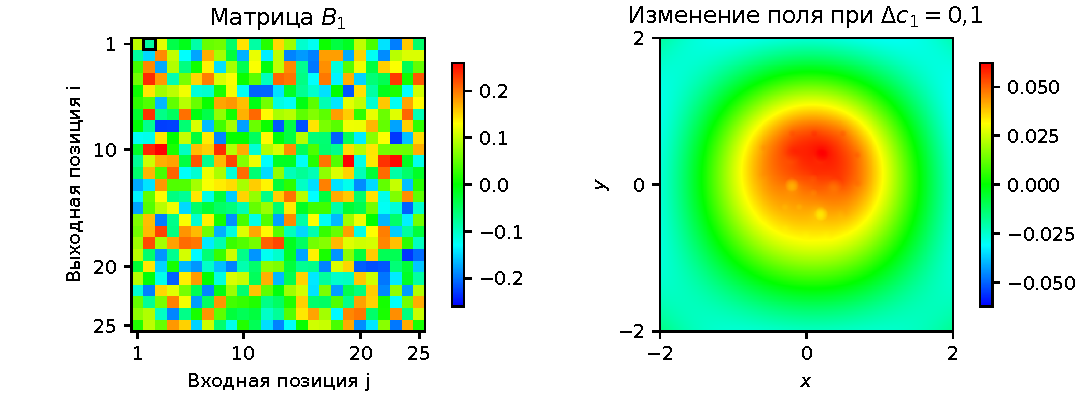
\includegraphics[width=.91\linewidth]{assets/operator_matrices.pdf}
\captionsetup{hypcap=false}\captionof{figure}{Слева оба индекса обозначают позиции
мод в первом блоке сети. Рамкой выделен вес $(B_1)_{1,2}$. Справа показано
изменение прогноза $0{,}1\phi_{1,R}(x)$ в физических координатах на эталонной сетке.
У каждой карты своя шкала с нулём в зелёном.}
\end{center}


\chapter{Один прогноз от параметров до значения в узле}
\label{walk:chapter}

Рассмотрим модель диапазона \texttt{low} из эксперимента
\mbox{\path{experiments/reference_sno_gmsfem}}. Её веса сохранены
на 497-й эпохе. Для одной среды
рассеянное поле рассчитывали методом конечных элементов на эталонной сетке
GMsFEM с $53\,246$ узлами и $105\,690$ треугольниками. Из 216 тестовых
полей выбираем то, чья относительная ошибка в норме $M$ ближе всего
к медиане. Это позиция~180 в массиве теста и индекс~940 во всём наборе
данных. Нумерация в обоих массивах начинается с нуля.

\section{Вход сети и первый блок}

Для снимка~940 волновое число $k=1{,}48616352$, угол
$\theta=3{,}30400881$ радиана. Среднее и стандартное отклонение $k$
на обучающей выборке равны $1{,}06892964$ и $0{,}53977354$.
При \mbox{$r_A=r_n=0$} вектор признаков~\eqref{code:feature-vector} равен
\[
 f=(\cos\theta,\sin\theta,\widetilde k)
    \approx(-0{,}9868395;\,-0{,}1617030;\,0{,}7729795).
\]
По критерию~\eqref{code:rank-criterion} с порогом $0{,}1\,\%$
получаем $E_V(24)\approx0{,}10121\,\%$ и $E_V(25)\approx0{,}05969\,\%$.
Поэтому $r_R=r_I=r_{\rm out}=25$ и $R=25$.
В каждой строке входной таблицы размера $25\times5$ стоит вектор
$(0,0,f_1,f_2,f_3)$. После входного слоя и GELU все строки
таблицы $Z_0\in\R^{25\times48}$ совпадают. Например, веса первого
канала при $f_1,f_2,f_3$ равны $-0{,}053747$, $0{,}226990$ и
$-0{,}049197$, а смещение равно $0{,}157807$. Сумма взвешенных
признаков и смещения составляет примерно $0{,}136114$. После GELU получаем
$(Z_0)_{j,1}\approx0{,}075425$ в каждой строке.

Пусть $z^\top$ --- общая строка $Z_0$. В глобальной ветви
первого блока $BZ_0 W_{\rm ch}=(B\bm 1)(z^\top W_{\rm ch})$.
Суммы первых двух строк матрицы $B$ равны $-0{,}015858$ и
$-0{,}344504$. Первый канал строки $z^\top W_{\rm ch}$ равен
$-0{,}048805$. Их произведения дают разные вклады глобальной ветви
в первый канал. Вклад локальной ветви в обеих строках равен
$0{,}124599$. По формуле~\eqref{code:block} получаем
\begin{align*}
 (Z_1)_{1,1}&\approx0{,}075425+\GELU(0{,}124599+0{,}000774)\approx0{,}144366,\\
 (Z_1)_{2,1}&\approx0{,}075425+\GELU(0{,}124599+0{,}016814)\approx0{,}154083 .
\end{align*}
Максимальное отклонение от первой строки
$\max_{j,h}|Z_{jh}-Z_{1h}|$ равно нулю до первого блока,
$0{,}973$ после первого блока и $17{,}444$ после шестого.
Размер таблицы остаётся $25\times48$ во всех шести блоках.
Выходной слой преобразует 48 каналов каждой строки в два
и выдаёт таблицу $\widehat q$ размера $25\times2$.

\clearpage
\section{Коэффициенты, узловое поле и его ошибка}

Первые три строки выхода сети и соответствующие коэффициенты POD
после пересчёта по формуле~\eqref{code:denormalize} приведены ниже.

\begin{center}
\begin{tabular}{@{}r rr rr@{}}
\toprule
& \multicolumn{2}{c}{Нормированные} & \multicolumn{2}{c}{После пересчёта}\\
\cmidrule(lr){2-3}\cmidrule(lr){4-5}
Мода $j$ & $\widehat q_{j,R}$ & $\widehat q_{j,I}$ &
 $\widehat c_{j,R}$ & $\widehat c_{j,I}$\\\midrule
1 & $-0{,}829477$ & $-0{,}931330$ & $-0{,}562294$ & $-0{,}706825$\\
2 & $-0{,}141463$ & $ 0{,}108413$ & $-0{,}094597$ & $ 0{,}067123$\\
3 & $-1{,}604440$ & $ 1{,}037706$ & $-0{,}948232$ & $ 0{,}525904$\\\bottomrule
\end{tabular}
\end{center}

У первого вещественного коэффициента среднее близко к нулю
($-3{,}59\cdot 10^{-16}$), а масштаб равен $0{,}677890$.
Умножение $-0{,}829477$ на этот масштаб даёт примерно $-0{,}562294$.

Ближайший к началу координат узел имеет индекс~27000 в массивах Python.
Значение первой вещественной моды в нём равно $0{,}50493962$.
Эта мода даёт вклад $0{,}50493962\cdot(-0{,}562294)\approx-0{,}28392452$,
остальные 24 моды дают в сумме $-0{,}04904686$. Прибавляем сумму
вкладов к среднему полю по~\eqref{code:decode-physical}. Для мнимой
части используем своё среднее и свои 25 мод.
\begin{align*}
 \widehat u_R(x_{27000})&\approx-0{,}21008244-0{,}33297133\approx-0{,}5430538,\\
 \widehat u_I(x_{27000})&\approx \phantom{-}0{,}63769776+0{,}37047899\approx1{,}0081768.
\end{align*}
Эталон в том же узле равен $-0{,}5444901+1{,}0092378\,\ii$.
Модуль прогноза равен $1{,}1451323$.

Для ошибки снимка нужны все $53\,246$ узловых значений.
Квадраты норм ошибки и эталонного поля вычисляем с согласованной
матрицей масс $M$.
\[
 \frac{\norm{\widehat u_s-u_s}_M}{\norm{u_s}_M}
 \approx \sqrt{\frac{9{,}07138\cdot10^{-5}}{5{,}89054}}
 \approx 0{,}3924\,\%.
\]
В архиве тестовых прогнозов ошибка снимка~940 равна $0{,}3924287\,\%$,
медиана по 216 полям --- $0{,}3924017\,\%$, средняя ошибка --- $0{,}7575\,\%$.
Все три числа относятся к рассеянному полю $u_s$.

\medskip
\textbf{Число обучаемых параметров.}
У входного слоя $5H$ весов и $H$ смещений. У каждого блока
$H^2+H$ параметров в локальной ветви, $H^2$ весов смешивания каналов
и $R^2$ весов смешивания позиций. У общего выходного слоя $2H$ весов
и два смещения. При $H=48$, $R=25$ и $L=6$ получаем
\[
 6H+L(2H^2+H+R^2)+(2H+2)=288+6\cdot5281+98=32\,072 .
\]

\clearpage
\section{Воспроизведение вычислений}

Запустите код из корня репозитория в окружении проекта. В каталоге
эксперимента он читает набор \mbox{\path{data/low}}, модель
\mbox{\path{runs/low/model.pt}} и массив тестовых ошибок \path{fem_l2}
из архива \mbox{\path{runs/low/test_predictions.npz}}.

\begin{lstlisting}
from pathlib import Path
import numpy as np
from experiments.reference_sno_gmsfem.dataset import load_dataset
from neural_operator.training import load_predictor

base = Path("experiments/reference_sno_gmsfem")
run = base / "runs/low"
with np.load(run / "test_predictions.npz") as saved:
    errors = saved["fem_l2"]
    position = int(np.argmin(abs(errors - np.median(errors))))
    sample = int(saved["indices"][position])

ds = load_dataset(base / "data/low")
p = load_predictor(run / "model.pt")
u = p.predict_dataset(ds, [sample])[0]
ref = ds.u_scat[sample]
node = np.argmin(np.linalg.norm(ds.coordinates, axis=1))

print(position, sample, node)
print(u[node], ref[node], abs(u[node]))
print(ds.relative_l2(ref, u), errors[position])
print(sum(w.numel() for w in p.model.parameters()))
\end{lstlisting}

В первой строке вывода будут индексы \texttt{180 940 27000}. Сверьте
узловые значения с расчётом выше. В третьей строке будут ошибки в
долях единицы, около $0{,}00392427$ и $0{,}00392429$ соответственно.
Последние цифры могут различаться при одиночном прогнозе и
при обработке пакета тестовых полей. В последней строке будет
число параметров \texttt{32072}.

\textbf{Проверка нормы на эталонной сетке.}
Вычислите числитель и знаменатель отдельно. Функция \path{np.vdot}
сопрягает первый аргумент, как требуется для комплексного поля.
\begin{lstlisting}
delta = u - ref
err2 = np.vdot(delta, ds.mass_matrix @ delta).real
ref2 = np.vdot(ref, ds.mass_matrix @ ref).real
print(err2, ref2, 100 * np.sqrt(err2 / ref2))
\end{lstlisting}
Получатся $9{,}07138\cdot10^{-5}$, $5{,}89054$ и $0{,}39243\%$.
Последнее число учитывает все треугольники эталонной сетки.

\chapter{Как читать численные результаты}
\label{exp:chapter}

В опыте \texttt{low} модель SVD-SNO v2 предсказывает рассеянное
поле в эталонной среде GMsFEM. На 216 тестовых запросах средняя
ошибка рассеянного поля составляет $0{,}7575\%$ относительно
эталонного решения методом конечных элементов (FEM).

\section{Задача, эталон и тестовые запросы}

Область $(-2,2)^2$ содержит 24 круговых включения. В фоне $A=n=1$,
во включениях $A=0{,}2$ и $n=10$. Для запроса $(k,\theta)$
систему~\eqref{math:fem-system} решают на P1-элементах исходной сетки
\path{gmsfem/meshes/reference_n20_h0p04.msh}. Её целевой шаг
$h=0{,}02$, число узлов $53\,246$, число треугольников $105\,690$.
Сохранены координаты, связность и порядок узлов эталона GMsFEM.
При $k=1$, $\theta=0$ повторный расчёт воспроизвёл эталонное поле
с относительным расхождением $9{,}1\cdot10^{-14}$.

К 160 значениям $k$, равномерно распределённым на $[0{,}1;2]$,
добавили $k=1$. Для каждой частоты взяли восемь направлений с шагом
$\pi/4$; начальный угол задан псевдослучайно, при $k=1$ он равен нулю.
Все восемь полей одной частоты попадают в одну выборку.
Группы $k=0{,}1$, $1$ и $2$ заранее отложены для теста.

\begin{table}[htbp]
\centering
\caption{Разбиение 1288 полей по частотам в опыте \texttt{low}.}
\label{exp:split}
\begin{tabular}{@{}lrrr@{}}
\toprule
 & Обучение & Валидация & Итоговый тест\\
\midrule
Значений $k$ & 107 & 27 & 27\\
Комплексных полей & 856 & 216 & 216\\
\bottomrule
\end{tabular}
\end{table}

При фиксированной среде входные POD-ранги $A$ и $n$ равны нулю.
Базисы и нормировки построены по обучающим полям. На валидации
выбраны выходной ранг и эпоха для сохранения весов. Тест проверяет
прогнозы для отложенных частот и направлений той же среды,
включая обе границы диапазона.

Для тестового запроса $q$ относительная ошибка рассеянного поля равна
\begin{equation}
 e_q=100\,\frac{\norm{\widehat u_{s,q}-u_{s,h,q}}_M}
                       {\norm{u_{s,h,q}}_M}\ \%,\qquad
 \norm{v}_M=\sqrt{v^*Mv}.
 \label{exp:metric}
\end{equation}
Матрица $M$ --- согласованная матрица масс эталонной сетки. Она
учитывает обе компоненты комплексной разности и даёт $L^2$-норму
кусочно-линейного поля.

\begin{table}[htbp]
\centering
\caption{Относительная комплексная ошибка рассеянного поля на
216 тестовых запросах. Среднее взято с одинаковым весом по запросам.}
\label{exp:stats}
\begin{tabular}{@{}rrrr@{}}
\toprule
Среднее & Медиана & 95-й процентиль & Максимум\\
\midrule
$0{,}7575\%$ & $0{,}3924\%$ & $2{,}6427\%$ & $6{,}0003\%$\\
\bottomrule
\end{tabular}
\end{table}

Около половины тестовых ошибок лежат ниже $0{,}3924\%$,
а около $95\%$ --- ниже $2{,}6427\%$. На отдельных запросах
отклонение от эталона достигает примерно $6\%$.

\clearpage
\section{Что сохраняют 25 мод в каждой компоненте}

По обучающим снимкам построены два вещественных POD-базиса,
отдельно для $\operatorname{Re}u_{s,h}$ и $\operatorname{Im}u_{s,h}$.
Использована рандомизированная SVD с диагональными весами узлов
$W=\diag(M\bm1)$. Перебор шёл до 96 мод на канал. Ранг 25 первым
достиг порога $0{,}1\%$ для средней ошибки проекции на валидации
по критерию~\eqref{code:rank-criterion}. Коэффициенты при этом
вычисляются с весами $W$, а ошибка измеряется в норме $M$.
В каждом канале декодер имеет вид $\mu+\sum_{j=1}^{25}a_j\phi_j$.

\begin{figure}[htbp]
\centering
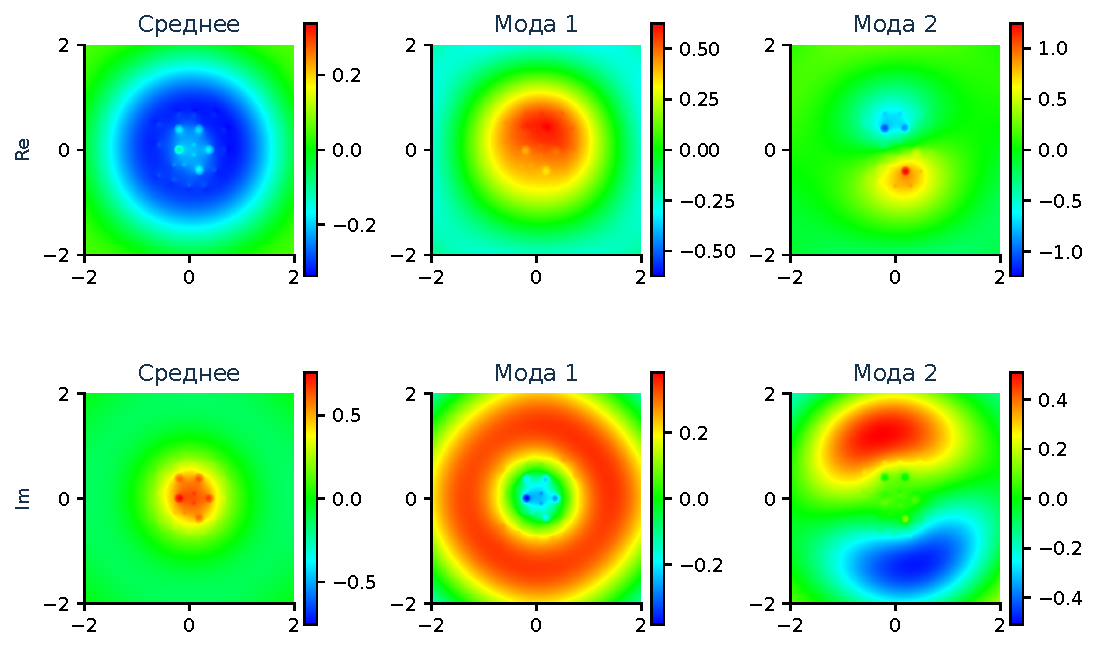
\includegraphics[width=.78\textwidth]{assets/pod_modes.pdf}
\caption{Обучающее среднее и первые две моды. Верхний ряд
соответствует вещественной части рассеянного поля, нижний --- мнимой.
У каждой карты своя шкала.}
\label{exp:modes}
\end{figure}

На верхней средней карте рисунка~\ref{exp:modes} изображена
$\phi_1$ вещественной части. Если увеличить её коэффициент на
$\delta>0$, поле в точке $x$ изменится на $\delta\phi_1(x)$.
Там, где мода жёлтая или красная, поле возрастёт, а где голубая или синяя,
уменьшится. Зелёный соответствует нулю. Смена знаков
у моды и её коэффициента сохраняет восстановленное поле.

\begin{figure}[htbp]
\centering
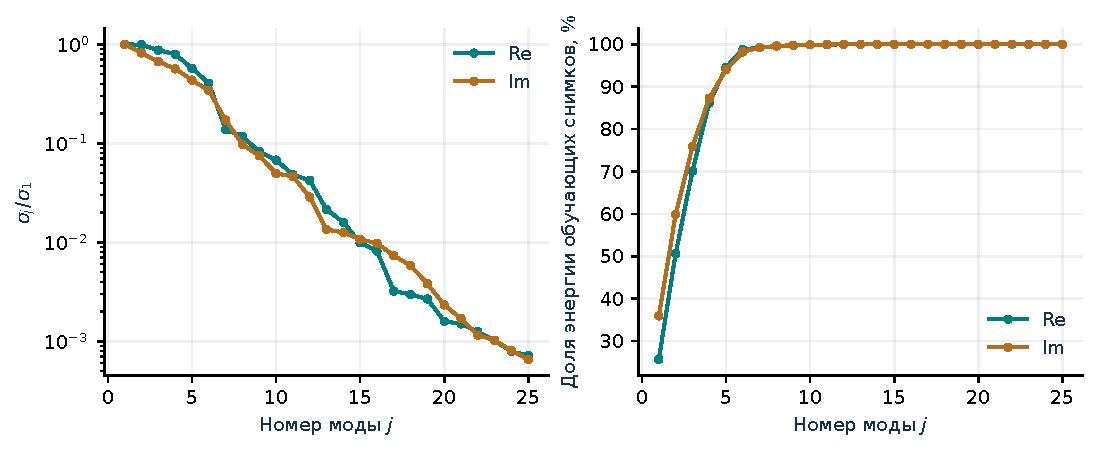
\includegraphics[width=.79\textwidth]{assets/spectrum.pdf}
\caption{Слева --- отношение $\sigma_j/\sigma_1$ в логарифмической шкале.
Справа --- накопленная доля энергии центрированных обучающих полей
в метрике $W$. Показаны сохранённые моды.}
\label{exp:spectrum}
\end{figure}

Числитель доли энергии на рисунке~\ref{exp:spectrum} равен
$\sum_{i=1}^j\sigma_i^2$, а знаменатель --- суммарной
$W$-энергии всех центрированных обучающих полей данного канала.
Для поля из отложенной выборки точность реконструкции проверяют
отдельно по формуле~\eqref{exp:metric}.

\clearpage
\section{Как отделить ошибку базиса от ошибки сети}

Для одного тестового поля сравним три способа получить
коэффициенты одного декодера. Проекция в норме $M$ решает нормальные
уравнения~\eqref{code:consistent-projection} и даёт наименьшую
ошибку для этого поля. Проекция в норме $W$ применяет
POD-кодирование~\eqref{code:pod-encoding}. Обе проекции требуют
значений эталонного поля. Сеть вычисляет коэффициенты по $k$ и
$\theta$, а эталон нужен для оценки прогноза.

\begin{figure}[htbp]
\centering
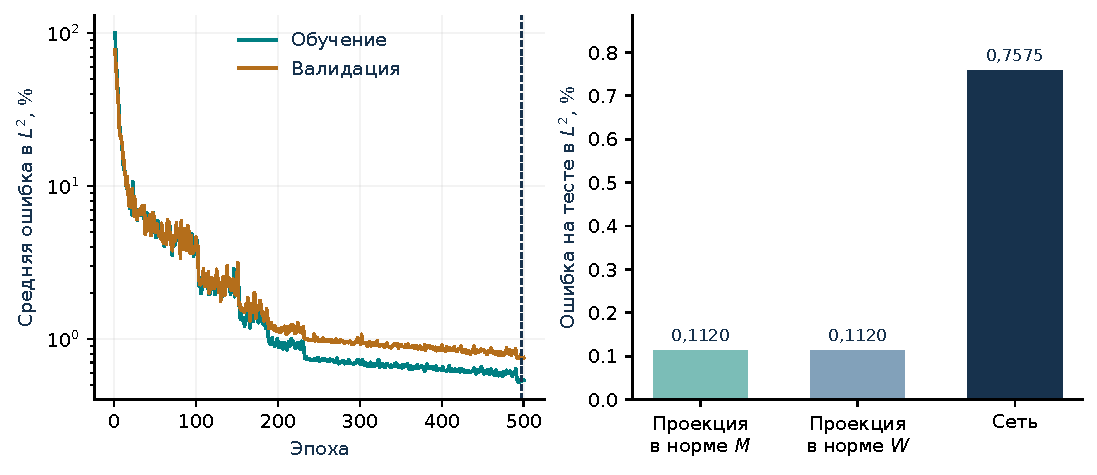
\includegraphics[width=.96\textwidth]{assets/training_and_floor.pdf}
\caption{Слева --- ошибки при обучении SVD-SNO v2 ширины 48,
с шестью блоками и 32\,072 обучаемыми параметрами. Справа ---
средние тестовые ошибки рассеянного поля в норме $M$
для трёх способов получить коэффициенты.}
\label{exp:history}
\end{figure}

На рисунке~\ref{exp:history} кривая «Обучение» усредняет ошибки
мини-пакетов по ходу эпохи. Кривая «Валидация» показывает ошибку с
весами на конец эпохи. При плато валидации шаг оптимизатора
уменьшался вдвое. Обучение дошло до лимита в 500 эпох. Пунктир
отмечает 497-ю эпоху, с которой взяты веса для тестирования.
Ей соответствует минимум валидационной ошибки $0{,}7390\%$.

Обе проекции в среднем дают $0{,}1120\%$ при округлении до четырёх
знаков после запятой. Сеть с тем же декодером даёт $0{,}7575\%$.

\begin{worked}{Какой выигрыш допускает фиксированный декодер?}
Можно ли получить среднюю ошибку $0{,}1\%$ на этих же тестовых
полях, улучшая лишь предсказание коэффициентов?

\textbf{Решение.} Оптимальная проекция эталонных полей даёт в среднем
$0{,}1120\%$. Этот минимум выше цели $0{,}1\%$, поэтому для неё
потребуется изменить пространство декодера. Разность между ошибкой сети
и минимумом составляет около $0{,}6455$ процентного пункта. Это разность
средних ошибок поля. Ортогональное сложение квадратов применяют
к каждому полю отдельно по формуле~\eqref{rig:projection-identity}.
\end{worked}

\clearpage
\section{Как читать карту одного прогноза}

На рисунке~\ref{exp:fields} показан тестовый снимок с ошибкой,
ближайшей к медиане. Его индекс в исходном наборе --- 940,
$k\approx1{,}48616$, $\theta\approx3{,}30401$ рад.
Относительная ошибка рассеянного поля составляет $0{,}3924\%$
с тем же округлением, что и в таблице~\ref{exp:stats}.

\begin{minipage}{\linewidth}
\centering
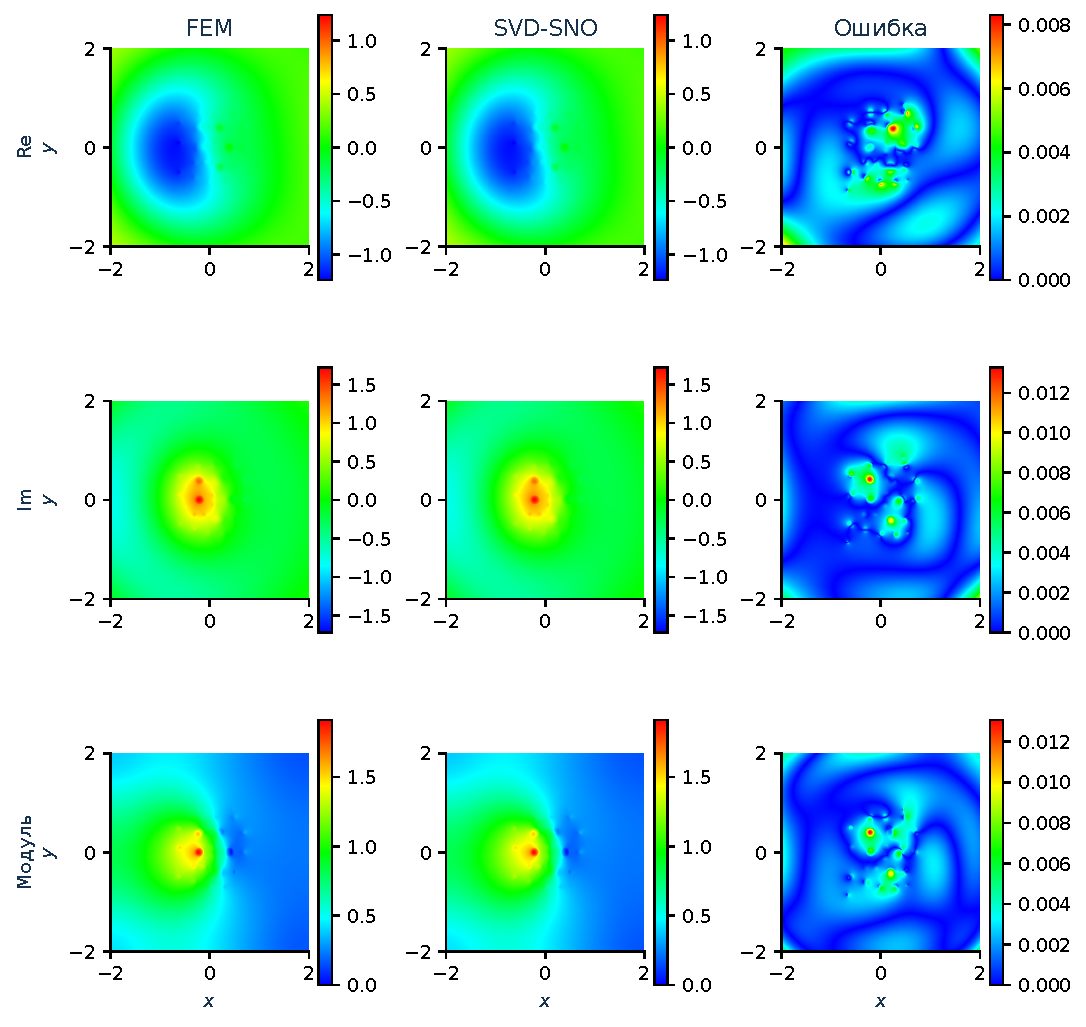
\includegraphics[width=.87\textwidth,height=.58\textheight,keepaspectratio]{assets/field_comparison.pdf}
\captionsetup{hypcap=false}\captionof{figure}{Рассеянное поле по МКЭ (FEM),
прогноз SVD-SNO и абсолютная ошибка. В каждом ряду поле и прогноз даны
в одной шкале, ошибка --- в собственной. Нуль на картах Re и Im поля и прогноза
выделен зелёным, на картах модуля и всех ошибок --- синим.}
\label{exp:fields}
\end{minipage}

Справа в первых двух строках показаны
$|\operatorname{Re}(\widehat u_s-u_{s,h})|$ и
$|\operatorname{Im}(\widehat u_s-u_{s,h})|$. Внизу справа показана
абсолютная разность модулей $\bigl||\widehat u_s|-|u_{s,h}|\bigr|$.
Внутри треугольника цвет определяется по линейной интерполяции узловых значений каждой карты.
Равенство модулей допускает ошибку фазы. Например, при
$\widehat u_s=-u_{s,h}$ нижняя правая карта всюду равна нулю,
а формула~\eqref{exp:metric} для ненулевого поля даёт $200\%$.

\clearpage
\section{Сравнение с GMsFEM на общих запросах}

Все методы в таблице~\ref{exp:comparison} проверены на одних и тех же
216 парах $(k,\theta)$. Рассеянные поля каждого метода вычисляют из
их собственных P1-представлений в точках семиточечной квадратуры
Дюнавана на эталонной сетке. К ним добавляют аналитическую падающую
волну~\eqref{math:incident}, чтобы получить полные поля.
Одна и та же падающая волна сокращается в разности, поэтому числитель
относительной комплексной ошибки совпадает для обоих полей.
Знаменатель берут отдельно для каждого эталона, $u_{s,h}$ и $u_i+u_{s,h}$.

\begin{table}[htbp]
\centering
\caption{Относительная комплексная $L^2$-ошибка в процентах
на общей квадратуре. Эталон --- FEM при $h=0{,}02$.}
\label{exp:comparison}
\begin{tabular}{@{}lrrrr@{}}
\toprule
 & \multicolumn{2}{c}{Рассеянное поле} & \multicolumn{2}{c}{Полное поле}\\
\cmidrule(lr){2--3}\cmidrule(l){4--5}
Метод & Среднее & 95-й перц. & Среднее & 95-й перц.\\
\midrule
SVD-SNO \texttt{low} & $0{,}7575$ & $2{,}6427$ & $0{,}3325$ & $1{,}1946$\\
FEM, $h=0{,}04$ & $0{,}1354$ & $0{,}3301$ & $0{,}0662$ & $0{,}2747$\\
GMsFEM $10\times10$, тип 1 & $3{,}1939$ & $11{,}6721$ & $1{,}9166$ & $9{,}7779$\\
GMsFEM $10\times10$, тип 2 & $1{,}4521$ & $4{,}2627$ & $0{,}7638$ & $3{,}6293$\\
GMsFEM $20\times20$, тип 1 & $1{,}7069$ & $6{,}6413$ & $1{,}0583$ & $5{,}5637$\\
GMsFEM $20\times20$, тип 2 & $0{,}5190$ & $1{,}2992$ & $0{,}2534$ & $1{,}1011$\\
\bottomrule
\end{tabular}
\end{table}

В этом тесте у GMsFEM $20\times20$ типа 2 ниже средние ошибки обоих
полей, чем у SVD-SNO. В каждой конфигурации GMsFEM использовано
по 16 локальных мод на вершину грубой сетки. Для каждого запроса метод
решает редуцированную физическую систему. SVD-SNO предсказывает
коэффициенты 25 глобальных мод в каждой компоненте. Поэтому число мод
означает разное для двух способов реконструкции.

В ошибку GMsFEM относительно эталона входят редукция и различие сеток.
Строка FEM при $h=0{,}04$ показывает межсеточную разницу после решения
полной системы на исходной сетке GMsFEM. Вычитание её
средней ошибки из ошибки GMsFEM даёт разность двух статистик,
а вклад редукции можно измерить прямым сравнением двух полей при
$h=0{,}04$.

\clearpage
\section{Что проверять при большой ошибке}

Обозначим через $u_s$ решение непрерывной задачи с поглощающим
условием, через $u_{s,h}$ --- его FEM-приближение, а через $u_*$ ---
проекцию $u_{s,h}$ в пространство декодера по норме $M$. Для
прогноза $\widehat u_s$ имеем
\[
 u_s-\widehat u_s
 =(u_s-u_{s,h})+(u_{s,h}-u_*)+(u_*-\widehat u_s).
\]
Первое слагаемое проверяют при уточнении FEM-сетки, сравнивая поля
в общих физических точках. Второе измеряют проекцией проверочных
FEM-полей в декодер. Третье измеряют сравнением прогноза с этой же
проекцией. При большом разрыве между ошибкой проекции и ошибкой
сети стоит проверить входные признаки, обратную нормировку
коэффициентов и порядок узлов при декодировании.

Два последних слагаемых ортогональны в норме $M$. Для оценки ошибки
относительно непрерывного решения требуется отдельно оценить
$u_s-u_{s,h}$. Измеренное сравнение двух сеток показывает изменение
FEM-решения между $h=0{,}04$ и $h=0{,}02$. Точность поглощающего
условия и перенос на новые среды требуют отдельных проверок.

Числа для SVD-SNO взяты из
\path{experiments/reference_sno_gmsfem/results/low/sno_metrics.json},
межсеточное сравнение --- из
\path{experiments/reference_sno_gmsfem/results/REPORT.md}.
Параметры показанного поля и происхождение измерений собраны в
\path{svd_sno_manual/assets/evidence.json}.

\chapter{Устойчивость и погрешность операторной модели}
\label{rig:chapter}
\label{op:chapter}

Пусть $p=(A,n,k,\theta)$ есть набор параметров. При единственности
решения усечённой краевой задачи ему соответствует рассеянное поле
$u_s(p)$. Так определяется оператор решения $\mathcal S:p\mapsto u_s(p)$.
Он вообще нелинеен по параметрам среды, хотя при фиксированных $A,n,k$
задача линейна по нагрузке. Конечно-элементный метод задаёт дискретный
оператор $\mathcal S_h:p\mapsto U(p)$, а обученная модель приближает
его значения. Возникают два вопроса. Насколько велика ошибка $U(p)$
относительно $u_s(p)$? Насколько близок к $U(p)$ прогноз по сокращённому
набору коэффициентов? Для ответов нужны разные нормы и разные константы.

\section{Устойчивость дискретной краевой задачи}
\label{rig:spaces}
\label{rig:discrete}

Пусть $\Omega$ есть ограниченная липшицева область, $k>0$, а $A,n$ ---
вещественные измеримые функции, для которых почти всюду
\begin{equation}
 0<A_{\min}\le A\le A_{\max}<\infty,\qquad
 0<n_{\min}\le n\le n_{\max}<\infty.\label{rig:coeff-bounds}
\end{equation}
Как и в главе~\ref{math:fem}, примем $A=1$ в окрестности
$\Gamma=\partial\Omega$. Введём пространство тестовых функций и норму
\begin{equation}
 V=H^1(\Omega;\C),\qquad \|v\|_{V,k}^2=\|\nabla v\|_{L^2}^2+k^2\|v\|_{L^2}^2.
 \label{rig:vnorm}
\end{equation}
В пространстве $V'$ непрерывных сопряжённо-линейных функционалов
норма нагрузки равна $\|\ell\|_{V',k}=\sup_{v\ne0}|\ell(v)|/\|v\|_{V,k}$.
Слабая форма и определяемый ею оператор имеют вид
\begin{equation}
 (\mathcal A_k w)(v)=a_k(w,v)
 =\int_\Omega A\nabla w\cdot\nabla\bar v
 -k^2\int_\Omega nw\bar v-\ii k\int_\Gamma w\bar v.\label{rig:form}
\end{equation}
Для решения выполняется $\mathcal A_k u_s=\ell$. Из неравенств
Коши--Буняковского и следа $\|v\|_{L^2(\Gamma)}\le C_{\rm tr}\|v\|_{H^1}$
следует оценка
\begin{equation}
 |a_k(w,v)|\le C_a(k)\|w\|_{V,k}\|v\|_{V,k},\qquad
 C_a(k)=A_{\max}+n_{\max}+k C_{\rm tr}^2\max(1,k^{-2}).\label{rig:continuity}
\end{equation}
С другой стороны, для ненулевой постоянной функции
$\operatorname{Re}a_k(v,v)=-k^2\int_\Omega n|v|^2<0$. Стандартное
доказательство устойчивости через положительную вещественную часть
здесь неприменимо.

Пусть $V_h\subset V$ есть пространство непрерывных кусочно линейных
функций на согласованной невырожденной триангуляции. В этой главе $u_{s,h}$
обозначает решение при точных интегралах. Тогда дискретная задача
задаётся равенством
\begin{equation}
 a_k(u_{s,h},v_h)=\ell(v_h)\quad(v_h\in V_h).\label{rig:galerkin}
\end{equation}
Нижнюю границу величины действия формы на единичном векторе задаёт число
\begin{equation}
 \beta_h(k)=\inf_{w_h\ne0}\sup_{v_h\ne0}
 \frac{|a_k(w_h,v_h)|}{\|w_h\|_{V,k}\|v_h\|_{V,k}},\qquad w_h,v_h\in V_h.
 \label{rig:beta}
\end{equation}
Константа зависит также от $A,n$. Положительность $\beta_h$ называется
дискретным условием inf-sup. В квадратной конечномерной системе она
равносильна обратимости.

\begin{theorem}[Оценка решения и ошибки по невязке]
При $\beta_h>0$ решение существует и единственно для каждой нагрузки.
Для приближения $v\in V_h$ положим $r_h(w_h)=\ell(w_h)-a_k(v,w_h)$.
Тогда
\begin{align}
 \|u_{s,h}\|_{V,k}&\le\beta_h^{-1}\|\ell\|_{V_h',k},\label{rig:discrete-stability}\\
 \|u_{s,h}-v\|_{V,k}&\le\beta_h^{-1}\|r_h\|_{V_h',k}.\label{rig:residual-estimate}
\end{align}
\end{theorem}
\begin{proof}
По \eqref{rig:beta} нулевой нагрузке может отвечать только нулевое
решение. Поэтому у квадратной системы тривиальное ядро и она обратима.
Подстановка решения в определение $\beta_h$ даёт первое неравенство.
Для второго достаточно применить его к задаче с решением $u_{s,h}-v$
и нагрузкой $r_h$.
\end{proof}

Пусть $L_h$ есть матрица системы \eqref{math:fem-system}, $K_0$ ---
матрица жёсткости при $A=1$ и $H_h=K_0+k^2M$. Вектор узловых значений
$z$ задаёт $\|z_h\|_{V,k}^2=z^*H_hz$. Для вектора нагрузки $F$
двойственная норма равна $(F^*H_h^{-1}F)^{1/2}$. Переход к переменным
$H_h^{1/2}z$ в \eqref{rig:beta} даёт
\begin{equation}
 \beta_h(k)=\sigma_{\min}(H_h^{-1/2}L_hH_h^{-1/2}).\label{rig:beta-matrix}
\end{equation}
Таким образом, одинаковая двойственная норма невязки может соответствовать
разным ошибкам при разных частотах. Для равномерного вывода нужна общая
положительная нижняя граница $\beta_h$ на рассматриваемом семействе.

\subsection{Возмущения сборки}
Пусть исходная система имеет вид $L_hU=F$, а вычисленная система ---
$(L_h+\Delta L_h)\widetilde U=F+\Delta F$. Обозначим
$\eta=\|H_h^{-1/2}\Delta L_hH_h^{-1/2}\|_2$, где $\|\cdot\|_2$ для
матрицы есть спектральная норма. При $\eta<\beta_h$ минимальное
сингулярное число нормированной возмущённой матрицы не меньше
$\beta_h-\eta$. Это следует из неравенства треугольника для
$(L_h+\Delta L_h)z$ в соответствующих нормах. Вычитая системы, получаем
правую часть $\Delta F-\Delta L_hU$ для разности решений и оценку
\begin{equation}
 \|\widetilde U-U\|_{H_h}
 \le\frac{\|\Delta F\|_{H_h^{-1}}+\eta\|U\|_{H_h}}{\beta_h-\eta}.
 \label{rig:operator-perturbation}
\end{equation}
Например, ошибка квадратуры одной только нагрузки входит через $\Delta F$.

\section{Переход от сетки к непрерывной задаче}
\label{rig:fem-convergence}

\begin{proposition}[Квазиоптимальность метода Галёркина]
Пусть $u_s\in V$ решает непрерывную задачу и $\beta_h>0$. Тогда при точном
интегрировании
\begin{equation}
 \|u_s-u_{s,h}\|_{V,k}\le
 \left(1+\frac{C_a(k)}{\beta_h(k)}\right)
 \inf_{v_h\in V_h}\|u_s-v_h\|_{V,k}.\label{rig:quasi-galerkin}
\end{equation}
\end{proposition}
\begin{proof}
Для любого $v_h\in V_h$ и любого теста $w_h$ имеем
$a_k(u_{s,h}-v_h,w_h)=a_k(u_s-v_h,w_h)$. Условия \eqref{rig:beta}
и \eqref{rig:continuity} дают
$\|u_{s,h}-v_h\|_{V,k}\le (C_a/\beta_h)\|u_s-v_h\|_{V,k}$.
Остаётся прибавить $\|u_s-v_h\|_{V,k}$ и взять инфимум.
\end{proof}
При фиксированной частоте для сходимости достаточно равномерной
устойчивости и условия $\inf_{v_h\in V_h}\|u_s-v_h\|_{V,k}\to0$ при $h\to0$.
В частности, на регулярных по форме треугольных сетках при $u_s\in H^2$
и максимальном диаметре элемента $h$ узловой интерполянт удовлетворяет
\begin{equation}
 \|u_s-I_hu_s\|_{V,k}\le C_I(h+kh^2)|u_s|_{H^2}.\label{rig:interpolation}
\end{equation}
Скачки свойств среды могут нарушить глобальную $H^2$-регулярность.
При изменении $k$ нужно учитывать также зависимость решения и $\beta_h$
от частоты.

Если фактические форма $a_h$ и нагрузка $\ell_h$ включают квадратуру,
возьмём любое приближение $v_h\in V_h$ и положим
$\psi_h(w_h)=\ell_h(w_h)-a_h(v_h,w_h)$. Пусть $\widetilde u_h$
решает фактическую задачу, а $\widetilde\beta_h>0$ есть её константа
устойчивости. Применяя \eqref{rig:residual-estimate} к
$\widetilde u_h-v_h$ и прибавляя ошибку аппроксимации, получаем
\begin{equation}
 \|u_s-\widetilde u_h\|_{V,k}\le\|u_s-v_h\|_{V,k}
                   +\widetilde\beta_h^{-1}\|\psi_h\|_{V_h',k}.
 \label{rig:consistency-residual}
\end{equation}
Здесь $v_h$ можно выбирать и при такой регулярности $u_s$, при которой
узловые значения самой функции не определены.

\section{Согласованная и диагональная матрицы массы}
\label{rig:mass-equivalence}

Для эрмитовых матриц запись $X\preceq Y$ означает
$z^*Xz\le z^*Yz$ при всех $z$. Связь между двумя метриками
главы~\ref{math:fem} особенно проста для линейных треугольников.

\begin{theorem}[Сравнение двух норм]
Для полной согласованной матрицы массы $M$ и $W=\diag(M\bm1)$ на
невырожденной треугольной сетке
\begin{equation}
 M\preceq W\preceq4M,\qquad
 \|z\|_M\le\|z\|_W\le2\|z\|_M.\label{rig:mass-bounds}
\end{equation}
\end{theorem}
\begin{proof}
На треугольнике площади $|T|$ имеем
$M_T=|T|(I+\bm1\bm1^\top)/12$, $W_T=|T|I/3$.
У постоянного вектора собственное значение $M_T$ равно $|T|/3$,
а у векторов с нулевой суммой координат оно равно $|T|/12$.
Следовательно, локально $M_T\preceq W_T\preceq4M_T$.
Суммирование локальных квадратичных форм по треугольникам даёт требуемые
неравенства, в том числе для комплексных $z$.
\end{proof}
Коэффициент 4 достигается уже на одном элементе. Результат относится
именно к полной линейной треугольной массе. Если имеются фиксированные
граничные значения, обе уже собранные формы можно ограничить на свободные
степени свободы. Повторное суммирование строк ограниченной $M$ даст другую
диагональную матрицу. Для элементов более высокого порядка нужны свои оценки.

\section{Наилучшее приближение в пространстве мод}
\label{rig:projection}

\begin{theorem}[Ортогональная проекция и ошибка коэффициентов]
Пусть $M=M^*>0$, $\mu\in\C^N$ и $\Phi\in\C^{N\times r}$ имеет
линейно независимые столбцы. Обозначим через $G=\Phi^*M\Phi$ матрицу
Грама и для $U\in\C^N$ определим
\begin{equation}
 Gc_*=\Phi^*M(U-\mu),\qquad P_MU=\mu+\Phi c_*,\qquad
 \rho=U-P_MU.\label{rig:projection-def}
\end{equation}
Тогда $P_MU$ есть единственное ближайшее к $U$ поле из
$\mu+\operatorname{ran}\Phi$, а при любом $c\in\C^r$
\begin{equation}
 \|U-\mu-\Phi c\|_M^2=\|\rho\|_M^2+\|c-c_*\|_G^2.
 \label{rig:projection-identity}
\end{equation}
\end{theorem}
\begin{proof}
Из независимости столбцов следует $x^*Gx=\|\Phi x\|_M^2>0$ при $x\ne0$.
Поэтому коэффициенты $c_*$ определены однозначно. По
\eqref{rig:projection-def} выполнено $\Phi^*M\rho=0$.
В разложении $U-\mu-\Phi c=\rho+\Phi(c_*-c)$ слагаемые
$M$-ортогональны, что даёт \eqref{rig:projection-identity}.
Его правая часть минимальна ровно при $c=c_*$.
\end{proof}
При $r=0$ пространство состоит из одного поля $\mu$ и остаётся только
остаток. Для раздельных вещественной и мнимой частей та же теорема
действует в $\R^{2N}$ с блочными матрицами $\diag(M,M)$ и
$\diag(\Phi_R,\Phi_I)$. При этом используют только независимые
активные столбцы каждой компоненты.

Пусть $P_W$ есть проекция на то же аффинное пространство в метрике $W$.
По минимальности обеих проекций и по \eqref{rig:mass-bounds}
\begin{equation}
 \|U-P_MU\|_M\le\|U-P_WU\|_M\le\|U-P_WU\|_W
 \le\|U-P_MU\|_W\le2\|U-P_MU\|_M.\label{rig:lumped-quasi}
\end{equation}
Таким образом, измеренная в $M$ ошибка $W$-реконструкции может превышать
оптимум. Её отношение к ненулевому оптимуму для этих элементов не больше двух.

\begin{worked}{Задача. Найдите обе проекции на одном треугольнике}
Пусть $|T|=1/2$, $U=(0,1,0)^\top$, а допустимые поля имеют вид
$(c,0,0)^\top$. Найдите коэффициент, дающий наименьшую ошибку в каждой
из норм.

\textbf{Решение.} Так как $W=I/6$, имеем $c_W=0$. Для полной матрицы
массы из \eqref{math:local-mass} уравнение проекции имеет вид
$(2/24)c_M=1/24$, откуда $c_M=1/2$. Квадрат $M$-ошибки для произвольного
$c\in\R$ равен $(2c^2-2c+2)/24$. При $c_W$ он равен $1/12$, при $c_M$
равен $1/16$. Соседние узловые функции перекрываются внутри элемента,
поэтому ненулевой коэффициент при первой функции улучшает приближение
второй в интегральной норме.
\end{worked}

\subsection{Почему SVD выбирает оптимальное пространство}
\label{rig:pod-optimality}
Для центрированных столбцовых снимков $S\in\C^{N\times m}$ и
$M=R^*R>0$ положим $Y=RS$. Любому $M$-ортонормированному базису
$\Psi\in\C^{N\times r}$ соответствует $Q=R\Psi$, причём $Q^*Q=I$.
Сумма квадратов ошибок проекции снимков равна
\[
 \|(I-QQ^*)Y\|_F^2=\operatorname{tr}(YY^*)-
                              \operatorname{tr}(Q^*YY^*Q).
\]
В собственном базисе $YY^*$ второй след равен $\sum_j\sigma_j^2p_j$.
Здесь спектр при необходимости дополнен нулями, а $p_j$ есть диагональные
элементы ортогонального проектора $QQ^*$ в этом базисе, так что
$0\le p_j\le1$ и $\sum_jp_j=r$. Максимум суммы достигается, когда весь
вес отведён первым $r$ собственным векторам. Следовательно, минимум
остатка равен $\sum_{j>r}\sigma_j^2$. Это доказывает оптимальность,
использованную в главе~\ref{math:pod}, и для комплексных снимков.
Если $m\ll N$, ненулевые квадраты сингулярных чисел находят по меньшей
матрице $Y^*Y=S^*MS$. Для нормированного собственного вектора $v_j$ и
$\sigma_j>0$ соответствующая мода равна $Sv_j/\sigma_j$.
Деление на очень малое $\sigma_j$ чувствительно к округлению.

\section{Чувствительность восстановления и сети}
\label{rig:decoder-stability}

Для декодера $D(c)=\mu+\Phi c$ квадрат нормы изменения поля равен
$\delta c^*G\delta c$. Поэтому при $r>0$
\begin{equation}
 \sqrt{\lambda_{\min}(G)}\,\|\delta c\|_2
 \le\|D(c+\delta c)-D(c)\|_M
 \le\sqrt{\lambda_{\max}(G)}\,\|\delta c\|_2.\label{rig:decoder-conditioning}
\end{equation}
При нормированных координатах $q$ и физическом векторе коэффициентов
$c=m_c+S_c q$ имеем
\begin{equation}
 \|D(m_c+S_c q_1)-D(m_c+S_c q_2)\|_M
 \le\underbrace{\|G^{1/2}S_c\|_2}_{\kappa_c}\|q_1-q_2\|_2.
 \label{rig:scaled-decoder}
\end{equation}
При $M$-ортонормированных модах $G=I$. Если ошибка затронула также
среднее и моды, $\widetilde D(c)=\mu+\delta\mu+(\Phi+\Delta\Phi)c$,
то из явной разности следует
\begin{equation}
 \|\widetilde D(c+\delta c)-D(c)\|_M
 \le\|\delta\mu\|_M+\|\Phi\delta c\|_M
 +\|\Delta\Phi\|_{2\to M}\|c+\delta c\|_2.
 \label{rig:decoder-perturb}
\end{equation}
Здесь $\|T\|_{2\to M}=\sup_{x\ne0}\|Tx\|_M/\|x\|_2$. Данная
чувствительность определяется пространством мод и масштабом коэффициентов.
Чувствительность решения краевой задачи задаёт другая константа, $\beta_h$.

\subsection{Как изменение признаков передаётся через сеть}
\label{rig:network-stability}
Для скрытых таблиц $Z$ используем норму Фробениуса. Один остаточный блок
действует как
\[
 F_\ell(Z)=Z+\alpha_\ell\sigma\bigl(ZW_{\rm loc}+\bm1 b^\top+
                                             B_\ell ZW_{\rm ch}\bigr).
\]
Пусть покомпонентная активация липшицева с константой $L_\sigma$.
Из $\|BZW\|_F\le\|B\|_2\|Z\|_F\|W\|_2$ и неравенства треугольника
следует
\begin{equation}
 \operatorname{Lip}(F_\ell)\le K_\ell=
 1+|\alpha_\ell|L_\sigma
 (\|W_{\rm loc}\|_2+\|B_\ell\|_2\|W_{\rm ch}\|_2).
 \label{rig:block-lip}
\end{equation}
Для синуса $L_\sigma=1$. Для точной GELU, $\sigma(t)=t\Phi_{\rm N}(t)$,
можно взять $L_\sigma=1+1/\sqrt{2\pi e}$, поскольку
$\sigma'(t)=\Phi_{\rm N}(t)+t\varphi_{\rm N}(t)$, где $\Phi_{\rm N}$ и
$\varphi_{\rm N}$ есть функция распределения и плотность стандартной
нормальной случайной величины.

В базовой архитектуре три общих признака повторяются в каждой из
$R_t=\max(r_{\rm out},r_A,r_n)$ строк. Каждый коэффициент материала
появляется один раз. Переход от плоского набора признаков к таблице
имеет норму $\sqrt{R_t}$. Если $W_{\rm in},W_{\rm out}$ есть матрицы
начального и выходного линейных слоёв, для сети из $L$ блоков имеем
\begin{equation}
 \operatorname{Lip}(N_\vartheta)\le\|W_{\rm out}\|_2
 \left(\prod_{\ell=1}^L K_\ell\right)
 L_\sigma\|W_{\rm in}\|_2\sqrt{R_t}.\label{rig:network-lip}
\end{equation}
Оценка учитывает активацию после входного слоя. Выбор первых выходных
строк имеет норму не больше единицы. Правая часть характеризует изменение
\emph{прогноза} между двумя входами. Для оценки его \emph{точности}
требуется сравнение с оператором решения.

\section{Аппроксимация оператора на семействе параметров}
\label{rig:identifiability}
\label{rig:total-error}

Определим модель на наборе параметров $\mathcal P$ формулой
\begin{equation}
 \widehat U(p)=D_h\!\left(m_c+S_cN_\vartheta(E_h(p))\right),\qquad
 p\in\mathcal P.\label{rig:factorized-model}
\end{equation}
Кодирование $E_h$ включает доступные сеточные признаки, их проекции
и нормировку. Детерминированная сеть выдаёт одинаковый ответ на два
запроса с одинаковым кодом. Если $E_h(p_1)=E_h(p_2)$, то для эталонов
$U_1,U_2$ на одной сетке
\begin{equation}
 \max_{j=1,2}\|U_j-\widehat U(p_j)\|_M\ge
                   \tfrac12\|U_1-U_2\|_M.\label{rig:input-floor}
\end{equation}
Действительно, расстояние между $U_1$ и $U_2$ не превосходит суммы
расстояний от них до их общего прогноза. Например, при нулевых входных
рангах два разных материала с одинаковыми $k,\theta$ получили бы один код.

\subsection{Разделение источников погрешности}
Пусть $c_*(p)$ и $\rho(p)$ есть коэффициенты и остаток точной $M$-проекции
эталона из \eqref{rig:projection-def}. Обозначим через $z(p)$ выбранные
идеальные признаки, через $\widehat z(p)$ --- фактически использованные
признаки. Для заданной функции $g$, сопоставляющей признакам нормированные
коэффициенты, положим
\begin{equation}
 a(p)=\|c_*(p)-m_c-S_c g(z(p))\|_G.\label{rig:representation-defect}
\end{equation}
Этот член учитывает точность самого описания через $g$ и $z$. При
неразличимых входах точное соответствие может оказаться невозможным.

\begin{proposition}[Оценка при заданных погрешностях звеньев]
Пусть $g$ липшицева с константой $L_g$ на множестве, содержащем
$z(p)$ и $\widehat z(p)$, и пусть в точке $p$ выполнены
$\|\widehat z-z\|_2\le\delta_z$,
$\|N_\vartheta(\widehat z)-g(\widehat z)\|_2\le\delta_N$.
Если вычисленный выход в нормированных координатах равен
$N_\vartheta(\widehat z(p))+e_q$, то для фиксированных среднего и мод
\begin{align}
 \|U(p)-\widehat U(p)\|_M
 &\le\sqrt{\|\rho(p)\|_M^2+Q(p)^2},\label{rig:end-to-end}\\
 Q(p)&=a(p)+\kappa_c\bigl(L_g\delta_z+\delta_N+\|e_q\|_2\bigr).\notag
\end{align}
\end{proposition}
\begin{proof}
В разности $\widehat c-c_*$ добавим и вычтем значения
$m_c+S_c g(z)$ и $m_c+S_c g(\widehat z)$. Неравенство треугольника,
условие Липшица и \eqref{rig:scaled-decoder} дают
$\|\widehat c-c_*\|_G\le Q(p)$. Остаётся применить точное тождество
\eqref{rig:projection-identity}.
\end{proof}
Если изменились также среднее и моды, к правой части добавляют
$\|\delta\mu\|_M+\|\Delta\Phi\|_{2\to M}\|\widehat c\|_2$. При
диагональной нормировке входов изменение одной координаты на $\delta y_j$
изменяет нормированную координату на $\delta y_j/s_j$. Поэтому малые
масштабы $s_j$ могут увеличить $\delta_z$.

Пусть $\widetilde u_h(p)$ есть конечно-элементная функция с эталонным
вектором $U(p)$, полученным при фактической сборке. Для перехода к
непрерывной задаче прибавляем $\|u_s(p)-\widetilde u_h(p)\|_{L^2}$
к оценке \eqref{rig:end-to-end}. Этот член включает погрешность
квадратуры. Его можно оценить по \eqref{rig:consistency-residual},
поскольку $\|v\|_{L^2}\le k^{-1}\|v\|_{V,k}$.
При сравнении с решением внешней задачи нужно учесть ещё ошибку
искусственной границы. Полученная величина относится к одному $p$.

\begin{idea}{Когда из оценки следует сходимость операторов}
Пусть все поля рассматриваются на общей области, а множество допустимых
параметров $\mathcal P$ фиксировано. Если при уточнении модели каждое
слагаемое приведённой абсолютной оценки стремится к нулю \emph{равномерно
по $p\in\mathcal P$}, то
$\sup_{p\in\mathcal P}\|u_s(p)-\widehat u_h(p)\|_{L^2}\to0$ для
усечённой задачи. Для равномерной относительной оценки достаточно также
границы $\inf_{p\in\mathcal P}\|u_s(p)\|_{L^2}>0$. Средняя ошибка на
конечном тестовом наборе характеризует только наблюдавшиеся запросы.
\end{idea}

\section{От математической нормы к вычисленной ошибке}
\label{rig:floating}
Вычисление \eqref{rig:projection-identity} в пространстве коэффициентов
позволяет заранее найти остатки и малую матрицу Грама. Для согласования
с фактическим декодером среднее и моды берут после округления до используемой
при восстановлении точности. Базовая реализация хранит их в одинарной
точности. Матрицу Грама, проекции и остатки по этим данным вычисляют
в двойной точности, причём остаток интегрируют непосредственно.
Это позволяет избежать вычитания двух почти равных энергий. При сравнении
с прямым восстановлением поля учитывают округления обеих процедур.

Если $e=\|U-\widehat U\|_M^2$ и $b=\|U\|_M^2$, базовая функция потерь
усредняет по примерам величину
\begin{equation}
 \ell_\varepsilon(e,b)=
 \frac{e}{\sqrt{\max(e,\varepsilon)}\sqrt{\max(b,\varepsilon)}},
 \qquad \varepsilon=10^{-24}.\label{rig:regularized-loss}
\end{equation}
При $e,b\ge\varepsilon$ это обычная относительная ошибка.
Вблизи $e=0$ такая запись даёт конечную производную по $e$ и сохраняет
нулевую потерю при точном прогнозе. Для почти нулевых полей результат
зависит от принятого правила. При чтении численных результатов нужно
уточнять, приведена ли ошибка по \eqref{math:relative-error} или значение
регуляризованной функции потерь.

\begin{worked}{Задача. Два запроса с одинаковым кодом}
Пусть два входа получили одинаковый код, а их эталонные поля равны
$\phi$ и $3\phi$, где $\|\phi\|_M=1$. Общий ответ имеет вид $t\phi$,
$t\in\R$. Какой ответ минимизирует наибольшую абсолютную ошибку?
Как изменится ответ, если ошибки считать относительно каждого эталона?

\textbf{Решение.} При $1\le t\le3$ абсолютные ошибки равны $t-1$ и
$3-t$. За пределами этого отрезка обе ошибки уменьшаются при движении
к нему. На отрезке максимум минимален при равенстве ошибок, то есть при
$t=2$. Он равен единице, что совпадает с нижней границей
\eqref{rig:input-floor}. Относительные ошибки равны $t-1$ и $(3-t)/3$.
Их равенство даёт $t=3/2$ и максимум $1/2$. Таким образом, переход к
относительной ошибке меняет оптимальный общий прогноз даже при тех же
полях и том же пространстве мод.
\end{worked}

\chapter{Один комплексный базис и несколько ветвей сети}
\label{adv:chapter}

Допустим, для семидесяти значений параметра уже вычислены комплексные поля.
Можно ли по ним восстановить поле при новом значении параметра?
Для ответа проведём два опыта. Сначала дадим алгоритму само проверочное
поле и попросим подобрать его координаты в обучающем базисе. Затем оставим
только параметры задачи и поручим подбор координат сети. Разница между
результатами покажет, на каком этапе теряется точность.

\section{Какие поля получает алгоритм}
\label{adv:family}

Один снимок $u_q\in\C^N$ содержит $N$ коэффициентов рассеянного поля
в конечноэлементном базисе одной сетки. Номер $q$ указывает на пару
$(k_q,\theta_q)$, где $k$ --- волновое число, а $\theta$ --- направление
падающей волны. Геометрия и материалы одинаковы для всех снимков.
В наборе \texttt{mscale\_sno\_100} зафиксирован также угол
$\theta=0$. Следовательно, изменяется один параметр, и приближаемая
зависимость имеет вид $k\mapsto u_h(k,0)$.

Всего в серии 100 решений при $k\in[0{,}1;4]$. Из них 70 отведены для
обучения, 15 для валидации (выбора весов сохранённой эпохи) и 15 для
итогового теста. Каждая сравниваемая модель получает одни и те же задачи.
Среднее поле, базис, его ранг и параметры нормировки определяются по 70
обучающим снимкам. Крайние значения $k$ входят в обучение, поэтому тест
проверяет интерполяцию по $k$ в одной среде.

\section{Как получить комплексные моды из снимков}
\label{adv:pod}

Пусть $v_h$ и $u_h$ --- конечноэлементные поля с векторами коэффициентов
$v$ и $u$. Их скалярное произведение $\int_\Omega\overline{v_h}u_h\,dx$
равно $v^*Mu$. Здесь $M_{ij}=\int_\Omega\psi_i\psi_j\,dx$ ---
согласованная матрица масс вещественного базиса $\{\psi_i\}$,
а звёздочка обозначает сопряжённое транспонирование. Матрица $M$
эрмитова и положительно определена. Она учитывает площадь элементов
и перекрытие базисных функций. Поэтому $\norm{u}_M^2=u^*Mu$
измеряет квадрат $L^2$-нормы пространственного поля, в том числе на
неравномерной сетке.

Вычтем из каждого обучающего поля комплексное среднее $\mu$ и запишем
отклонения в столбцы матрицы $S$:
\[
 \mu=\frac1n\sum_{q=1}^n u_q,\qquad
 S=[u_1-\mu,\ldots,u_n-\mu]\in\C^{N\times n},\qquad n=70.
\]
Сумма столбцов равна нулю, поэтому их ранг не превосходит $69$.
Среднее сохраняется отдельно. Для поиска мод достаточно решить
собственную задачу размера $70\times70$:
\begin{equation}
 G=S^*MS=V\Lambda V^*,\qquad
 \Phi_R=SV_R\Lambda_R^{-1/2}.
 \label{adv:gram}
\end{equation}
Здесь $V_R$ содержит собственные векторы, соответствующие $R$ наибольшим
численно положительным собственным значениям $\lambda_j$.
Формула имеет простую проверку по размерам. Матрица $V_R$ размера
$n\times R$ задаёт смеси снимков, а $S V_R$ размера $N\times R$ уже
задаёт пространственные поля. Деление каждого столбца на
$\sqrt{\lambda_j}$ нормирует его. Подставив \eqref{adv:gram}, получим
$\Phi_R^*M\Phi_R=I_R$.

При точной арифметике $\lambda_j$ --- вклады мод в суммарную энергию
отклонений $u_q-\mu$. Код отбрасывает численные нули и ищет минимальное
$R$, для которого
\begin{equation}
 \frac{\sum_{j>R}\lambda_j}{\sum_j\lambda_j}\leq 10^{-8},
 \label{adv:energy}
\end{equation}
с верхним пределом $R\leq60$. Если предел достигнут раньше порога,
остаётся максимально допустимый ранг. В этом опыте хватило \textbf{17 мод}.
После построения базиса код корректирует его ортонормированность малым
разложением Холецкого. Условие \eqref{adv:energy} относится к сумме
квадратов отклонений обучающих полей. Относительную ошибку отдельного
нового поля ещё предстоит измерить.

\section{Проверка базиса до обучения сети}
\label{adv:loss}

Возьмём известное поле $u$ из тестовой выборки. Его наилучшие координаты
в метрике $M$, проекция и остаток равны
\[
 a_* = \Phi_R^*M(u-\mu),\qquad
 u_* = \mu+\Phi_R a_*,\qquad r=u-u_* .
\]
Проекция оставляет от $u-\mu$ ровно ту часть, которую можно выразить
через моды. Действительно, $\Phi_R^*Mr=0$. Для произвольного прогноза
$\widehat u=\mu+\Phi_R\widehat a$ из этого следует
\begin{equation}
 \norm{u-\widehat u}_M^2
 =\underbrace{\norm{r}_M^2}_{\text{остаток базиса}}
 +\underbrace{\norm{a_*-\widehat a}_2^2}_{\text{ошибка координат}}.
 \label{adv:pyth}
\end{equation}
Первое слагаемое одинаково для всех сетей с данным декодером. Второе
можно измерить, даже не восстанавливая $N$ значений прогноза.
При $u\ne0$ деление суммы на $\norm{u}_M^2$ и извлечение корня дают
относительную ошибку поля. При обучении усредняют эти ошибки по примерам.

\begin{worked}{Практикум. Проверьте проекцию с комплексным коэффициентом}
Пусть $M=I_2$, $\mu=0$, $\phi=(1,\ii)^T/\sqrt{2}$ --- единственная
сохранённая мода, а $u=(0,1)^T$. Найдите наилучшую реконструкцию и
ошибку сети, если сеть вернула $\widehat a=0$.

\textbf{Решение.} Сопряжение даёт $a_*=\phi^*u=-\ii/\sqrt{2}$, откуда
$u_*=(-\ii,1)^T/2$. Остаток $r=(\ii,1)^T/2$ имеет квадрат нормы $1/2$,
причём $\phi^*r=(\ii-\ii)/(2\sqrt{2})=0$. Ошибка координаты добавляет ещё $1/2$.
Поскольку $\norm{u}_2=1$, относительная ошибка наилучшей проекции равна
$1/\sqrt2$, а прогноза --- $1$. Поле $\widehat u=0$ даёт тот же ответ
при непосредственной проверке.
\end{worked}

Для проверки реализации удобно обработать сразу несколько проверочных
полей. В следующем фрагменте строка \texttt{U[q]} --- одно поле,
\texttt{Phi} имеет форму \texttt{(N, R)}, а \texttt{M} --- разреженная
матрица масс. В строке восстановления сопряжения нет.
\begin{lstlisting}
centered = U - mean
coeff = (M @ centered.T).T @ Phi.conj()
projected = mean + coeff @ Phi.T
residual = U - projected
gram = Phi.conj().T @ (M @ Phi)
orthogonality = (M @ residual.T).T @ Phi.conj()
\end{lstlisting}
Матрица \texttt{gram} должна быть близка к единичной, а
\texttt{orthogonality} --- к нулевой в пределах точности вычислений
и масштаба полей. Эти два теста помогают обнаружить перепутанные оси,
пропущенное сопряжение или матрицу масс от другой сетки.

\section{Как ветви предсказывают координаты}
\label{adv:architecture}

При новом запросе известны только $k$ и $\theta$. Сеть получает вектор
$x=((k-\bar k)/s_k,\cos\theta,\sin\theta)$, где $\bar k$ и $s_k$ ---
обучающие среднее и стандартное отклонение $k$. В рассматриваемой серии
последние два признака равны 1 и 0 для всех примеров.

Ветвь $j$ умножает все три признака на свой обучаемый скаляр $c_j$.
Её первый слой переводит $c_j x$ в $R W$ чисел. Мы укладываем их в
таблицу $Z$ с $R$ строками по числу мод и $W$ столбцами по числу скрытых
признаков. Уже после первого слоя у каждой моды своя строка. После
нелинейности применяются $D$ блоков вида
\[
 Z\ \longleftarrow\ Z+D^{-1/2}
 \rho\!\left(ZL+\mathbf1 b^T + BZC\right).
\]
Матрицы $L,C\in\R^{W\times W}$ преобразуют признаки, $b\in\R^W$ задаёт
смещение, а $B\in\R^{R\times R}$ смешивает строки разных мод. У каждого
блока и ветви свои веса. В многоветвевой модели $\rho=\sin$.
Ветви начинают обучение с разными $c_j$, поэтому изменение $k$ подаётся
на их входы в разных масштабах.
Пространственное разрешение во всех ветвях задаётся одной матрицей $\Phi_R$.

Выходной слой каждой ветви превращает строку из $W$ чисел в пару
$(\operatorname{Re}p_{jr},\operatorname{Im}p_{jr})$ для моды $r$.
Результат всей сети и поле имеют вид
\[
 s_a=\sqrt{\frac{1}{nR}\sum_{q=1}^n\sum_{r=1}^R|a_{qr}|^2},\qquad
 \widehat a_r=s_a\sum_{j=1}^J\gamma_j p_{jr},\qquad
 \widehat u=\mu+\Phi_R\widehat a.
\]
Единый масштаб $s_a$ возвращает нормированные выходы в физические единицы.
Веса $\gamma_j$ изначально равны $1/J$ и затем обучаются без ограничения
на сумму. Среднее $\mu$ добавляется один раз, после сложения ветвей.

\begin{worked}{Проверка размеров и числа параметров}
Подсчитаем веса одной ветви. Первый слой с тремя входами и смещением
требует $4RW$ параметров. Один блок содержит $2W^2+W+R^2$, выходной
слой --- $2W+2$. Добавим $c_j$ и $\gamma_j$. При $R=17$, $W=8$, $D=4$
получаем $544+4(128+8+289)+18+2=2264$ параметра.
У восьми ветвей их $18\,112$, а выход по-прежнему состоит из $17$
комплексных коэффициентов. Сеть с одной ветвью и подобранной шириной
в этом сравнении имеет $18\,380$ параметров.
\end{worked}

\clearpage
\section{Что показали пятнадцать тестовых полей}
\label{adv:comparison}

В таблице~\ref{adv:results} все три запуска используют один базис и те же
15 тестовых задач. Номер запуска служит начальным значением генератора,
от которого зависят начальные веса и порядок примеров при обучении.
В каждом запуске взяты веса эпохи с наименьшей средней ошибкой
на валидации. Числа в таблице --- проценты относительной комплексной
$L^2$-ошибки рассеянного поля по формуле~\eqref{exp:metric}. Для каждой строки
сначала вычислена ошибка каждого снимка, затем взяты соответствующие статистики.

\begin{table}[htbp]
\centering
\caption{Восьмиветвевая модель. Меньшее значение означает более точное поле.}
\label{adv:results}
\begin{tabular}{@{}lrrr@{}}
\toprule
Номер запуска & Среднее, \% & 95-й процентиль, \% & Максимум, \%\\
\midrule
11 & 65,85 & 84,55 & 85,26\\
29 & 60,96 & 87,84 & 89,87\\
47 & 60,19 & 94,58 & 96,14\\
\bottomrule
\end{tabular}
\end{table}

При координатах из истинных тестовых полей средняя ошибка того же
декодера равна всего $0{,}01579\%$. Значит, пространство ранга 17
хорошо представляет именно эти поля. Разрыв с таблицей указывает на
неточность предсказанных координат. Из чисел нельзя установить, как
разделить её между влиянием объёма выборки и процедурой обучения.

Для сравнения возьмём одну ветвь с той же синусоидальной активацией
и близким числом параметров. При начальных значениях 11, 29 и 47
её средние ошибки составили соответственно $71{,}15\%$, $74{,}99\%$
и $69{,}64\%$. Во всех трёх запусках восемь ветвей уменьшили среднюю
ошибку. Эти три наблюдения относятся к одной и той же тестовой выборке.

Общий эталон для этих запросов --- FEM-поля на сетке с $h\approx0{,}02$.
На той же квадратуре средняя ошибка FEM с шагом $h=0{,}04$ составила
$1{,}0170\%$, а у четырёх вариантов GMsFEM она лежала между $6{,}8244\%$
и $31{,}3606\%$. Средняя ошибка каждого запуска сети оказалась выше.
Все эти сравнения относятся к одним и тем же 15 физическим запросам.

\begin{worked}{Вопрос по таблице}
Верно ли, что запуск 47 дал самый точный результат для каждой частоты?
\textbf{Решение.} У запуска 47 наименьшее среднее, но наибольший
максимум. На частоте, где его ошибка достигла $96{,}14\%$, оба других
запуска дали меньшую ошибку: даже их максимумы ниже. Чтобы узнать,
на каких ещё частотах меняется порядок, нужны попарные ошибки по снимкам.
\end{worked}

Данные для воспроизведения таблицы находятся в
\path{experiments/mscale_sno_100/results/summary.csv}, а проекционные
остатки --- в \path{results/training_summary.json} той же серии.
Модули \texttt{pod.py} и \texttt{model.py} с реализациями базиса и ветвей
находятся в \path{experiments/gms_sno_100/}.

\clearpage
\section{Что проверяет смена сетки}
\label{adv:mesh}

\textbf{Вычисление уже полученного поля в новых точках.}
Для непрерывного кусочно-линейного поля (P1) пусть $T$ переводит
исходные узловые значения в значения в новых точках внутри сетки
с помощью барицентрической интерполяции. Линейность даёт
\[
 T(\mu+\Phi_R a)=T\mu+(T\Phi_R)a .
\]
Значит, среднее и моды можно перенести один раз, а затем подставлять
новые коэффициенты. Равенство правой и левой частей --- проверка порядка
узлов и корректности реализации переноса. Оно выполняется даже при
большой ошибке исходного поля относительно решения уравнения.

\textbf{Сравнение решений на двух сетках.}
Здесь нужны два решения одной физической задачи. Для исследования влияния
сетки на весь метод заново строят FEM-метки, базис и модель на каждой
сетке при одинаковых физических запросах. Следует сравнивать декодированные
поля в одних физических точках и интегрировать разность на общей
проверенной квадратуре. Даже на одной сетке моду можно домножить на
$e^{\ii\alpha}$ и компенсировать фазу в коэффициенте. Поэтому разность
модальных координат из двух независимых базисов сама по себе малоинформативна.

В сеточном пилоте проекта для $k=20$ различия квадратичных FEM-решений
между последовательными уровнями составили $5{,}40\%$ и $0{,}50\%$.
В этих числах участвуют только FEM-поля. Для вывода о сеточной
устойчивости сети нужны предсказания на обеих сетках и их сравнение
с общим эталоном. Особенно важно разделять эти проверки при повышении
$k$, когда пространственная сетка должна разрешать более короткие волны.

\textbf{Изменение диапазона параметра.}
Для новой обучающей серии могут измениться и формы полей, и их нормы.
Например, в высокочастотной серии проекта ранг выбирается по
среднеквадратической относительной ошибке проекции на обучающих полях,
$\big(n^{-1}\sum_q \|u_q-u_{*,q}\|_M^2/\|u_q\|_M^2\big)^{1/2}$.
Здесь каждое поле входит со своим знаменателем. Доля общей
центрированной энергии в \eqref{adv:energy} сильнее зависит от снимков
с большими отклонениями от среднего. Правило выбора ранга и метрику
проверки следует указывать вместе с числом оставленных мод.

\chapter{Справочник и литература}
\label{sources:chapter}

\section{Обозначения, к которым удобно вернуться}
\begin{center}
\renewcommand{\arraystretch}{1.18}
\begin{tabularx}{\linewidth}{@{}l X@{}}
\toprule
Обозначение & Смысл \\ \midrule
$p=(A,n,k,\theta)$ & Один запрос: свойства среды, волновое число и угол падения.\\
$u_i,\ u_s,\ u_{s,h}$ & Падающее, рассеянное и приближённое рассеянное поля.\\
$N,\ m,\ r$ & Число узлов, число обучающих снимков, число оставленных мод.\\
$U,\ \widehat U$ & Векторы узловых значений расчётного поля и прогноза.\\
$\varphi_i,\ \phi_j$ & Узловая функция МКЭ и пространственная POD-мода.\\
$\mu,\ \Phi_r,\ c$ & Среднее поле, матрица из $r$ мод и модальные коэффициенты одного поля.\\
$M,\ W$ & Согласованная матрица масс и её диагональное приближение. Определяют два скалярных произведения на одной сетке.\\
$T,\ *$ & Верхние индексы матрицы: транспонирование и сопряжённое транспонирование. Для вещественных матриц совпадают.\\
\bottomrule
\end{tabularx}
\end{center}

\section{Где посмотреть реализацию}
Пути ниже отсчитываются от корня репозитория. Основной код расположен
в \path{neural_operator/}. Для чтения конкретной формулы достаточно
открыть соответствующий файл.

\begin{center}
\begin{tabularx}{\linewidth}{@{}l X@{}}
\toprule
Файл в \path{neural_operator/} & Что искать \\ \midrule
\path{fem.py}, \path{data.py} & Сборка системы МКЭ, нагрузка, матрица масс и норма поля.\\
\path{sno/basis.py} & Среднее, взвешенное SVD, переход от поля к коэффициентам и обратно.\\
\path{sno/model.py}, \path{_layers.py} & Входная таблица признаков, смешивание мод и выходные коэффициенты.\\
\path{losses.py} & Квадратичная форма для оценки ошибки по коэффициентам.\\
\path{training.py} & Подготовка базисов, выбор ранга, обучение и загрузка модели.\\
\bottomrule
\end{tabularx}
\end{center}
В серии \path{experiments/reference_sno_gmsfem/} файл \path{dataset.py}
открывает эталон GMsFEM, а \path{training.py} задаёт цикл обучения SVD-SNO.
Для комплексного варианта см.\ \path{experiments/gms_sno_100/pod.py}
и \path{model.py} в том же каталоге. Описание опыта со 100 полями
находится в \path{experiments/mscale_sno_100/METHOD.md}.

\clearpage
\section{Литература для самостоятельного чтения}
\begin{enumerate}[itemsep=.45em]\RaggedRight
\item В.\,С. Фанасков, И.\,В. Оселедец. \emph{Спектральные нейронные операторы}.
Доклады РАН. Математика, информатика, процессы управления, 514(2),
72--79 (2023). В развёрнутой англоязычной работе архитектуру описывают
раздел 4 и приложение C.1.3. \href{https://www.mathnet.ru/rus/danma452}{Русская статья},
\href{https://arxiv.org/html/2205.10573v2}{англоязычная версия},
\href{https://github.com/VLSF/SNO/tree/4362226284f22f6f456d429ec4ddec5b8596e894}{авторская реализация}.
\item C. Eckart, G. Young. \emph{The Approximation of One Matrix by Another of
Lower Rank}.\newline Psychometrika, 1, 211--218 (1936). Исходная работа об
оптимальном приближении матрицы заданного ранга.
\href{https://doi.org/10.1007/BF02288367}{DOI 10.1007/BF02288367}.
\item L. Sirovich. \emph{Turbulence and the Dynamics of Coherent Structures.
I. Coherent Structures}. Quarterly of Applied Mathematics, 45, 561--571
(1987). Построение мод по корреляциям снимков.
\href{https://doi.org/10.1090/qam/910462}{DOI 10.1090/qam/910462}.
\item N. Halko, P.-G. Martinsson, J.\,A. Tropp.
\emph{Finding Structure with Randomness}. SIAM Review, 53, 217--288 (2011).
Как случайная выборка помогает приближённо выделить ведущее
сингулярное подпространство. \href{https://arxiv.org/abs/0909.4061}{Полный текст авторов}.
\item Z. Li и др. \emph{Fourier Neural Operator for Parametric Partial
Differential Equations} (2020). Параметризация оператора в пространстве
Фурье. \href{https://arxiv.org/abs/2010.08895}{arXiv:2010.08895}.
\item L. Lu и др. \emph{A Comprehensive and Fair Comparison of Two Neural
Operators (with Practical Extensions) Based on FAIR Data}. Computer Methods
in Applied Mechanics and Engineering, 393, 114778 (2022). Варианты
DeepONet, в том числе с выходным POD-базисом.
\href{https://arxiv.org/abs/2111.05512}{Полный текст авторов}.
\item А.\,А. Самарский. \emph{The Theory of Difference Schemes} (2001).
Общие понятия аппроксимации и устойчивости разностных схем.
\href{https://www.routledge.com/The-Theory-of-Difference-Schemes/Samarskii/p/book/9780429208171}{Издание на английском языке}.
\end{enumerate}

\section{Как повторить примеры и собрать пособие}
Из корня проекта в его Python-окружении выполните
\begin{lstlisting}[language=bash]
python svd_sno_manual/build_notation_assets.py
python svd_sno_manual/build_assets.py
python svd_sno_manual/check_sno_examples.py
python svd_sno_manual/mini_demo.py
sh svd_sno_manual/build.sh
\end{lstlisting}
Первые две команды работают с сохранённым расчётом на эталонной сетке
и повторяют прогноз без переобучения. Следующие две проверяют алгебру
слоя и функции потерь. Для сборки PDF достаточно готовых иллюстраций,
XeLaTeX и шрифтов, перечисленных в \path{svd_sno_manual/README.md}.

\end{document}
